 \documentclass [14pt]{extreport}
 \usepackage[cp1251]{inputenc}
 \usepackage[ukrainian]{babel}
 \usepackage{latexsym}
 \usepackage{graphicx}
 \usepackage{float}
 \usepackage{epsfig}
 \usepackage{lipsum}
 \usepackage{euscript}
 \usepackage{amsmath, amssymb}
 \usepackage[hidelinks]{hyperref}
 \textwidth16.7cm
 \textheight22.7cm
 \textwidth15.5cm
 \textheight22cm
 \topmargin0cm
 \evensidemargin0cm
 \lefthyphenmin=2
 \righthyphenmins=3
 \leftmargin=1.1cm
  \rightmargin=1.5cm
\renewcommand{\baselinestretch}{1.8}
 \renewcommand{\arraystretch}{0.6}
\renewcommand{\theequation}{\thechapter.\arabic{equation}}
 \renewcommand{\bibname}{Список використаних джерел}
 \newcommand\real{{\rm I\! R}}
 \newcommand\cmplx{\;\hbox{\vrule height6.8pt width0.8pt %depth-0.1pt
           \kern-3.6pt {\rm C}}}
 \newcommand\nat{{\rm I\! N}}
 \newcommand\integer{{\rm Z \!\! Z}}
 \newcommand\abs{\par\noindent}
 \newcommand\smalf{\par\smallskip\noindent}
 \newcommand\medlf{\par\medskip\noindent}
 \newcommand\biglf{\par\bigskip\noindent}
 \renewcommand{\thetheorem}{\thesection}
 \renewcommand{\thesection}{\thechapter.\arabic{section}.}
 \newcommand\thesec1{\thechapter .\arabic{section}}
\renewcommand{\thesubsection}%
{\thesection\arabic{subsection}.}
 \newtheorem{theorem}{Теорема}[section]
 \renewcommand{\chapter}{\centerline{{Розділ}[chapter]}
 \renewcommand{\thetheorem}{\thesection\arabic{theorem}}
 \newtheorem{definition}[theorem]{Означення}
 \newtheorem{lemma}[theorem]{Лема}
 \newtheorem{remark}[theorem]{Зауваження}
 \newcommand\proof{{\noindent \it Доведення.\ }}
 \newcommand\beweis{\ \hfill$\Box$}
 \newcommand\beweisende{\ \hfill$\Box$\break}
 \newtheorem{kor}[theorem]{Corollary}
\newtheorem{lem}[theorem]{Lemma}
\newtheorem{remark}[theorem]{Remark}
\newcommand\re{\mathop{\rm Re}\nolimits}
\newcommand\im{\mathop{\rm Im}\nolimits}
\newcommand\Dex{\real^2\setminus\Gamma}
\newcommand\Dexab{\real^3\setminus D}
\newcommand\Grad{\mathop{\rm Grad}\nolimits}
\newcommand\Div{\mathop{\rm Div}\nolimits}
\newcommand\grad{\mathop{\rm grad}\nolimits}
\newcommand\sinc{\mathop{\rm sinc}\nolimits}
\newcommand\divv{\mathop{\rm div}\nolimits}
\newcommand\curl{\mathop{\rm curl}\nolimits}
\newcommand\ar{\!\!\!\!}
\newcommand\vkappa{{\gamma}}
 \def\bql#1{\begin{equation}\label{#1}}
 \def\bq{\begin{equation}}
 \def\eq{\end{equation}}
 \def\eref#1{{\rm (\ref{#1})}}
 \def\btr{\begin{theorem}\hspace{-1.8mm}{\bf.}\hspace{3mm}}
 \def\ble{\begin{lemma}\hspace{-1.8mm}{\bf.}\hspace{3mm}}
 \def\bdf{\begin{definition}\hspace{-1.8mm}%{\bf.}\hspace{3mm}}
\DeclareRobustCommand{\bbone}{\text{\usefont{U}{bbold}{m}{n}1}}
\DeclareMathOperator{\EX}{\mathbb{E}}
% **************************************************************************
 \includeonly{titel,vstup,rozdil_1,rozdil_2,rozdil_3,vysnovok,bibl}

% ***************************************************************************
 \begin{document}
 \pagestyle{myheadings}
 \flushbottom
% **************************************************************************
 \thispagestyle{empty}
\renewcommand{\baselinestretch}{1}

\Large
\begin{center}
Міністерство освіти і науки України \\
Львівський національний університет імені Івана Франка \\
Факультет прикладної математики та інформатики \\
Кафедра математичного моделювання соціально-економічних процесів
\end{center}

\vspace*{2cm}
\begin{center}
\huge Дипломна Робота
\end{center}

\vspace*{1cm}
\large
\begin{center}
\textbf{Онлайн графічний рушій з фізично обґрунтованим моделюванням освітлення} \\
\end{center}
\vspace*{1cm}
\normalsize

\vspace*{1.5cm}
\noindent
\hspace*{8.6cm}Студент групи ПМА-42: \\
\hspace*{8.6cm}\textbf{Коломієць Даніїл Васильович}, \\
\hspace*{8.6cm}спеціальність 124-системний аналіз

\vspace*{0.5cm}
\noindent
\hspace*{8.6cm}Науковий керівник: \\
\hspace*{8.6cm}кандидат фізико-математичних наук, \\
\hspace*{8.6cm}доцент \\
\hspace*{8.6cm}\textbf{Лисецька Олександра Юріївна}

\vspace*{0.0cm}
\noindent

\vspace*{1.5cm}
\large
\begin{center}
Львів--2024
\end{center}
\normalsize
\renewcommand{\baselinestretch}{1.3}
\tableofcontents
% **************************************************************************
  \markright{\underline{\it Вступ}}

% \renewcommand{\baselinestretch}{1.3}
 \normalsize
 \chapter*{Вступ}
 \addcontentsline{toc}{chapter}{Вступ}
 %\large
У сучасному світі комп’ютерна графіка відіграє надзвичайно важливу роль. Вона присутня практично в кожному аспекті нашого цифрового життя: від інтерфейсів 
користувача на мобільних пристроях і комп’ютерах — до високобюджетного кінематографа та відеоігор. У багатьох випадках графіка використовується для візуалізації
 інформації або об'єктів без потреби в достовірному фізичному відтворенні взаємодії світла з матеріалами, як-от у веб-додатках чи користувацьких інтерфейсах. 
 Проте у сферах, де реалізм є ключовим — таких як віртуальна реальність, ігри чи CGI у фільмах — фізично коректне моделювання освітлення стає необхідністю. Саме
  від нього залежить глибина занурення глядача у віртуальний світ.

\par Реалістичне зображення не може бути досягнуте без розуміння та імітації фізичних процесів взаємодії світла з поверхнями. 
Однак комп’ютерна графіка стикається з низкою фундаментальних труднощів: фізичні явища є неперервними за своєю природою, а комп’ютери оперують 
дискретними структурами даних. Наприклад, постають питання, як описати складну геометрію тіла людини, як ефективно її візуалізувати, або як забезпечити
 правдоподібний рух цих об'єктів у просторі.

\par У цій науковій роботі увага буде зосереджена на одному з найважливіших аспектів — моделюванні фізично обґрунтованого освітлення. 
Інші компоненти графічного рушія, такі як геометричне моделювання чи анімація, будуть розглядатися лише побіжно або ігноруватимуться, оскільки 
метою роботи є реалізація та дослідження саме цього напряму.
 

% ***************************************************************************
 % *********************** Це є Розділ 1 ************************************

 \markright{\underline {\it Розділ 1. Постановка задачі}}

 \setcounter{chapter}{0}
 \chapter{Моделювання фізично правильної взаємодії світла }

 
 \par У цьому розділі приведено визначенно основних терміні та визначенно основні проблеми, пов'язані з моделюванням фізично правильної взаємодії світла з 
      об'єктами в комп'ютерній графіці. 

 \section{Людське сприйняття зображень}
  \setcounter{equation}{0}
 \setcounter{theorem}{0}

 \par Перед тим як вдаватись до деталей моделювання фізично правильної взаємодії світла з об'єктами, важливо розглянути, 
 яким чином людське оке сприймає світло та як мозок формує зображення.
 \par Світло - це квантова елетромагнітна хвиля, швидкість якої рівна \\ $299\,792\,458\,\text{m/s}$. Видимий спектр світла знаходиться між 
 380 та 780 наномет\-рами рис. \ref{fig:LightSpectrum}. Видимо світло яке є монохромним відповідає деякему кольору спектру. Зазвичай джерела світла випромінюють 
 світло в широкому діапазоні довжин хвиль. Наприклад денне світло є суперпозицією деякого діапазону хвиль рис. \ref{fig:LightSuper}.
Спостерігати ми це можемо під час веселки, коли світло проходить через краплі води, розкладаючись на спектр кольорів.

 \begin{figure}[h]
  \centering
  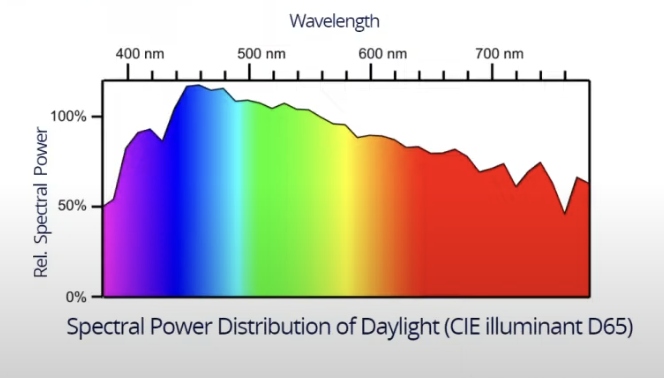
\includegraphics[scale=1]{Pictures/LightSuper.png}
  \caption{Спектральний розподіл енергії денного світла}
  \label{fig:LightSuper}
\end{figure}

\begin{figure}[h]
\centering
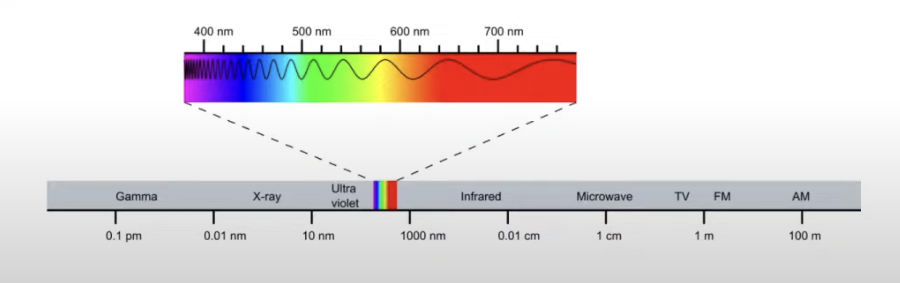
\includegraphics[scale=1]{Pictures/LightSpec.png}
\caption{Видимий спект світла}
\label{fig:LightSpectrum}
\end{figure}

  \par Світло також взаємодіє з навколишніми об'єктами. Припустимо, що світло випромінюється деяким джерелом в однорідних речовинах, наприклад повітрі
  світло рухається по прямій, деякі промені світла можуть попасти одразу в людське око, інші ж потрапляють на деякі об'єкти, які в свою чергу поглинають, відбивають або
  пропускають фотони світла. Відповідно до цього, ми можемо спостерігати різні кольори об'єктів, які залежать від того, які довжини хвиль світла вони відбивають.
  Те світло яке потрапляє в око людини, проходить через рогівку, кришталик та склоподібне тіло, де воно фокусуються на сітківці ока. Сітківка містить фоторецептори, 
  які реагують на світло і перетворюють його в електричні сигнали, що надсилаються до мозку. Мозок обробляє ці сигнали і формує зображення, яке ми сприймаємо.

 \begin{figure}[h]
  \centering
  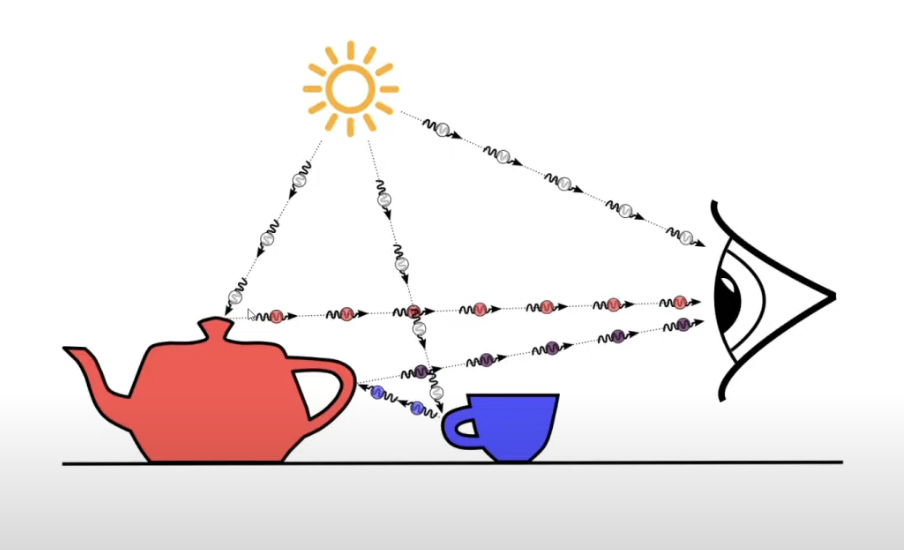
\includegraphics[scale=1]{Pictures/LightPath.png}
  \caption{Шлях світла від джерела до ока людини}
  \label{fig:LightPath}
\end{figure}

\par
Загалом у людини існують дві основні системи фоточутливих рецепторів, що забезпечують зорове сприйняття:
\begin{enumerate}
\item \textbf{Палички} — фоторецептори, які мають високу чутливість до інтенсивності світла та забезпечують зір при слабкому освітленні 
(скотопічний зір). Вони не розрізняють кольори.
\item \textbf{Колбочки} — рецептори, відповідальні за кольоровий (фотопічний) зір. Вони чутливі до різних діапазонів довжин хвиль електромагнітного 
випромінювання. Існує три типи колбочок рис. \ref{fig:LightRecept}:
\begin{enumerate}
    \item \textbf{L-колбочки} (Long) — реагують на довгі довжини хвиль (приблизно 560–580 нм), що відповідає червоному діапазону спектра.
    \item \textbf{M-колбочки} (Medium) — сприймають середні довжини хвиль (приблизно 530 нм), асоційовані із зеленим кольором.
    \item \textbf{S-колбочки} (Short) — чутливі до коротких довжин хвиль (приблизно 420–440 нм), які відповідають синьому кольору.
\end{enumerate}
\end{enumerate}

 \begin{figure}[h]
  \centering
  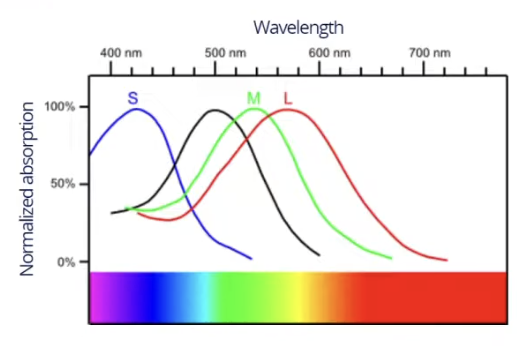
\includegraphics[scale=1]{Pictures/LightRecept.png}
  \caption{Людські колбочки та діапазон їх чутливості}
  \label{fig:LightRecept}
\end{figure}

Через те, що людське око має лише три типи колбочок, людське око не може сприймати реальний спектральний розподіл енергії світла,
завдяки цьому око можна обманювати, і різні спектрані розподіли енергії світла можуть сприйматись як однакові кольори. Саме через це, в комп'ютерній графіці
застосовується RGB кольорова модель, де R-red(червоний) G-green(зелений) B-blue(синій). Змішуючи ці три кольори в різних пропорціях, можна отримати 
більшість кольорів, які сприймаються людським оком рис \ref{fig:RGB}. Прямий фізичний зв'язок між спектральним розподілом енергії світла та RGB описано в \cite{Ch0} та \cite{Ch1}.
Більшість сучасних моніторів та екранів використовують sRGB кольорову модель для відображення зображень, але для фізично правильного рендерингу треба працювати в 
лінійному спектрі, для цього застосовується так звана \textit{гама корекція}, яка дозволяє перетворити кольори з sRGB в лінійний спектр \cite{Ch2}.
Основна ідея, яку слід засвоїти, полягає в тому, що немає потреби симулювати транспортування світла для кожної довжини хвилі окремо. Для більшості практичних застосувань 
достатньо розраховувати перентранспортуванняесення світла для трьох основних кольорів. Це значно спрощує обчислення та робить задачі 
рендерингу обчислювально ефективнішими.

\begin{figure}[h]
  \centering
  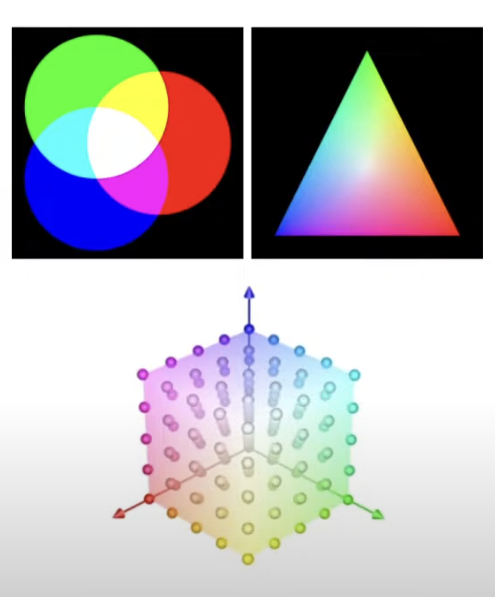
\includegraphics[scale=1]{Pictures/RGB.png}
  \caption{RGB кольорова модель}
  \label{fig:RGB}
\end{figure}

 \section{Визначення рівняння Рендерингу}
   \setcounter{equation}{0}
 \setcounter{theorem}{0}

 \subsection{Радіометричні величини}

Перш ніж дати визначення рівнянню рендерингу, варто розглянути деякі основні фізичні величини, які в ньому зустрічаються. Одним із базових понять є \textit{тілесний кут}.

\par
У школі ми вивчали поняття кута у двовимірному просторі. Щоб визначити, який кут охоплює об’єкт з певної точки спостереження, уявімо коло з центром у цій точці та проектуємо об’єкт на коло. Кут визначається як відношення довжини дуги $s$ до радіуса $r$:
\[
\theta = \frac{s}{r}
\]
Оскільки кут є безрозмірною величиною, його вимірюють у радіанах. 
\par
У тривимірному просторі аналогом звичайного кута є \textit{тілесний кут} (англ. \textit{solid angle}). Щоб визначити тілесний кут, який охоплює об’єкт з певної точки, розмістимо у цій точці центр уявної сфери та проектуємо об’єкт на її поверхню. Тілесний кут визначається як відношення площі проєкції $s$ до квадрата радіуса сфери:
\[
\omega = \frac{s}{r^2}
\]
Це також безрозмірна величина, яку вимірюють у \textit{стеррадіанах (sr)}. Повна сфера має тілесний кут $4\pi$ стеррадіан.

\par
Для обчислення тілесного кута, що покриває певну область, його розбивають на нескінченно малі елементи $d\omega$ і інтегрують по всій області:
\[
\omega = \int d\omega
\]

\par
Зручним способом параметризації є сферичні координати, які задаються двома кутами: полярним кутом $\theta$ (від $0$ до $\pi$) та азимутальним кутом $\phi$ (від $0$ до $2\pi$). Нескінченно мала ділянка тілесного кута виражається через поверхневий елемент $ds$:
\[
d\omega = \frac{ds}{r^2}
\]
Припускаючи, що радіус $r = 1$, обчислимо $ds$ як площу елемента поверхні сфери:
\[
ds = \sin{\theta} \, d\theta \, d\phi
\]
Таким чином, фінальна формула для нескінченно малої ділянки тілесного кута набуває вигляду:
\[
d\omega = \sin{\theta} \, d\theta \, d\phi
\]

А загальна формула для тілесного кута, що охоплює певну область на сфері, виглядає так:
\bql{eq:SolidAngle}
\omega = \int_0^{2\pi} \int_0^{\pi} \sin{\theta} \, d\theta \, d\phi
\eq

\paragraph{Потік випромінювання (Radiant Flux).}
Потік випромінювання, або \textit{radiant flux}~$\Phi$, — це енергія електромагнітного випромінювання, що передається в одиницю часу:
\[
\Phi = \frac{dQ}{dt}
\]
де $Q$ — енергія, $t$ — час. Одиниця вимірювання — ват (Вт), тобто джоуль на секунду (Дж/с).

Кожен фотон несе енергію
\[
E = \frac{hc}{\lambda}
\]
де $h$ — стала Планка, $c$ — швидкість світла, $\lambda$ — довжина хвилі.

Таким чином, потік випромінювання можна інтерпретувати як сумарну енергію фотонів, що випромінюються джерелом світла за одиницю часу. У графіці $\Phi$ 
використовується для опису загального випромінювання точкового джерела.

\paragraph{Інтенсивність випромінювання (Radiant Intensity).}
Інтенсивність випромінювання $I$ — це потік випромінювання на одиницю тілесного кута:
\[
I = \frac{d\Phi}{d\omega}
\]
Одиниця вимірювання — Вт/ср (ват на стеррадіан). Ця величина використовується, коли джерело випромінює нерівномірно в різних напрямках, як, наприклад, 
у випадку прожектора. Для точкового джерела, що випромінює рівномірно у всіх напрямках:
\[
I = \frac{\Phi}{4\pi}
\]

\paragraph{Опроміненість (Irradiance).}
Опроміненість $E$ — це потік випромінювання, що потрапляє на одиницю площі поверхні:
\[
E = \frac{d\Phi}{dA}
\]
Одиниця — Вт/м$^2$. Потік може надходити з усіх напрямків півсфери над поверхнею. Для нескінченно малої ділянки $dA$, яку 
освітлює точкове джерело, враховується тілесний кут $d\omega$, під яким джерело бачиться з цієї ділянки. Якщо $\theta$ — кут між нормаллю до 
поверхні та напрямком на джерело, то проєкція враховується через множник $\cos{\theta}$:

\[
E = \frac{I \cdot \cos{\theta}}{r^2}
\]

де $r$ — відстань до джерела.

Оскільки $I = \frac{\Phi}{4\pi}$, то для точкового джерела маємо:
\[
E = \frac{\Phi \cdot \cos{\theta}}{4\pi r^2}
\]

Це показує, що опроміненість спадає з квадратом відстані та залежить від кута падіння світла.

\paragraph{Енергетична яскравість (Radiance).}
Енергетична яскравість $L$ визначається як потік випромінювання, що проходить через одиницю площі в певному напрямку, на одиницю тілесного кута:
\[
L = \frac{d^2\Phi}{dA_{\perp} \, d\omega}
\]
де $dA_{\perp} = \cos{\theta} \, dA$ — проєкція площі в напрямку потоку. Одиниця — Вт/(м$^2$·ср).
Ця величина не залежить від відстані до джерела, адже при зменшенні відстані тілесний кут збільшується, але площа яка спостерігається - зменшується.
Спостергіти це явище ми можемо на прикладі стіни, змінючи відстань до неї, ми можемо спостерігати що яскравість стіни не змінюється.

\paragraph{Зв'язок між опроміненістю та енергетичною яскравістю.}
Опроміненість можна визначити через інтегрування енергетичної яскравості по всій півсфері $\Omega_h$ напрямків над поверхнею:
\bql{eq:RadianceToIrradiance}
E = \int_{\Omega_h} L(\omega) \cos{\theta} \, d\omega
\eq

\subsection{Рівняння рендерингу}
Рівняння рендерингу описує, як світло взаємодіє з поверхнями об'єктів і як це впливає на зображення, яке ми бачимо. Воно базується на фізичних принципах 
передачі світла та його взаємодії з матеріалами.
\bql{eq:RenderingEquation}
  L_o(\mathbf{v}) = L_e(\mathbf{v}) + \int_{\Omega_h} f_r(\mathbf{v},\mathbf{l} ) L_i(\mathbf{l}) \cos{\theta} d\omega
\eq

де: $L_o(\mathbf{v})$ — вихідна енергетична яскравість у напрямку $\mathbf{v}$, $L_e(\mathbf{v})$ — енергетична яскравість, що випромінюється поверхнею в напрямку $\mathbf{v}$,
$f_r(\mathbf{v},\mathbf{l})$ — \textit{Двопроменева функція розподілу відбивної здатності}(BRDF), що описує, як світло знапрямком $\mathbf{l}$ відбивається від 
поверхні в напрямок $\mathbf{v}$, $L_i(\mathbf{l})$ — вхідна енергетична яскравість у напрямк)у $\mathbf{l}$, 
$\theta$ — кут між нормаллю до поверхні та напрямком на джерело світла, $d\omega$ — тілесний кут.\\
Якщо придивитися уважно, то можна побачити, що рівняння рендерингу містить в собі рівняння для опроміненості \eref{eq:RadianceToIrradiance}.
\paragraph{Складність обчислення рівняння освітлення.}

Інтегрування по всій півсфері напрямків~$\Omega_h$ означає врахування всіх можливих напрямків поширення світла, яке може впливати на задану точку поверхні.
 Це робить рівняння освітлення обчислювально складним, адже для кожної точки сцени потрібно проінтегрувати внесок світла з усіх напрямків півсфери, орієнтованої 
 відносно нормалі до поверхні.

Кожен об’єкт у сцені сам по собі є джерелом випромінювання, тобто володіє певною вихідною енергетичною яскравістю в довільному напрямку~$\mathbf{v}$. Взаємне 
освітлення між об’єктами створює глобальну взаємозалежність, де світло, відбите від однієї поверхні, може впливати на інші поверхні, і так далі — потенційно нескінченну
 кількість разів.

Складність посилюється тим, що будь-яка поверхня є неперервною\footnote{Поверхня та кількість світлових променів у сцені є скінченними, проте їхня кількість настільки велика, 
що варто вважати їх нескінченними та неперервними} множиною точок, а з кожної точки в нескінченну кількість напрямків можуть надходити фотони. На 
мікроскопічному рівні поверхні не ідеально гладкі: вони можуть мати шорсткості, мікрогеометрію, відмінні оптичні властивості (наприклад, металічність, діелектричність,
 шорсткість тощо), що впливають на спосіб взаємодії зі світлом.

Оскільки світло може багаторазово відбиватися між поверхнями перед тим, як потрапити в камеру або око спостерігача, точне симулювання всіх траєкторій кожного 
фотона є обчислювально недосяжним\footnote{Існують методи, такі як Ray Tracing та Path Tracing, які симулюють поведінку світла, але лише для скінченної кількості променів, та
малої кількість відбитів світла від поверхонь} завданням для сучасних комп’ютерів.

У зв’язку з цим, замість точного моделювання всіх траєкторій, у комп’ютерній графіці застосовуються стохастичні методи, які описують розповсюдження світла у вигляді
 ймовірнісного процесу. Зокрема, розглядається ймовірність того, що промінь світла з певного напрямку~$\mathbf{l}$, взаємодіючи з поверхнею з відомими матеріальними 
 властивостями, буде відбитий в інший напрямок або поглинутий. Саме BRDF функція дозволяє моделювати цю ймовірність, і давати загальне уявлення про те, як світло
взаємодіє з поверхнею.\\
Варто зауважити, що такий підхид не дає точного рішення рівняння рендерингу, але дозволяє отримати
достатньо реалістичні результати за розумний час. У комбінації з іншими методами, такими як трасування променів, глобальне освітлення та інші,
можна досягти високої якості зображень, які виглядають фізично коректно, хоча і не є абсолютно точними.




% ***************************************************************************
 % *********************** Це є Розділ 2 ************************************

 %\markright{\underline {\it Розділ 2. Теоретичне рішення проблеми}}

 %\setcounter{chapter}{1}
 \chapter{ТЕОРЕТИЧНЕ ВИРІШЕННЯ ПРОБЛЕМИ}

 
 У цьому розділі розглядається теоретичне підґрунтя розв'язання задачі рендерингу в рамках створення власного графічного рушія. Спочатку описується 
 базовий процес рендерингу геометрії, далі розглядаються моделі BRDF, що визначають фізично коректне відбиття світла від поверхонь, а також методи оптимізації, 
 які забезпечують ефективну роботу системи в реальному часі.

\section{Рендеринг геометрії}
  \setcounter{equation}{0}
 \setcounter{theorem}{0}
 Рендеринг геометрії є фундаментальною складовою комп’ютерної графіки й одночасно однією з найскладніших задач. Безпосереднє математичне описання складних форм (наприклад, анатомії людини) аналітичними функціями практично неможливе, тому використовуються чисельні апроксимації. Найпоширеніший підхід полягає в розбитті поверхні на набір елементарних багатокутників, зазвичай -- трикутників. Така триангуляція дозволяє будь–який многовид наближати довільно точно, регулюючи щільність сітки.

Графічний процесор (GPU) оптимізований під ефективну обробку саме трикутних сіток. Кожен трикутник задається трьома вершинами та відповідними індексами ребер. GPU приймає буфери вершин і індексів, виконує трансформації та проєкцію, а потім передає дані далі в конвеєр -- тобто в pipeline.

\subsection*{Графічний конвеєр і шейдери}
Графічний пайплайн складається з кількох етапів:
\begin{enumerate}
    \item \textbf{Вершинний шейдер (Vertex Shader)} -- застосовує афінні пе\-рет\-во\-рен\-ня до вершин: поворот, масштаб, перенесення та проєкцію у відсічений об’єм.
    \item \textbf{Тесселяція (опціонально)} -- процес динамічного розбиття примітивів (переважно трикутників або чотирикутників), що формують геометрію об'єктів, на менші  з метою підвищення рівня деталізації. 
      
    \item \textbf{Геометричний шейдер (Geometry Shader)} -- може додатково генерувати чи модифікувати примітиви на основі вхідних даних.
    \item \textbf{Растеризація} -- перетворює примітиви (трикутники) у фрагменти (пік\-се\-лі), відсікає ті, що знаходяться поза областю перегляду.
    \item \textbf{Фрагментний (піксельний) шейдер (Fragment / Pixel Shader)} -- обчислює колір кожного фрагмента з урахуванням матеріальних влас\-ти-\-вос\-тей і текстур.
    \item \textbf{Тест глибинності й блендінг} -- вирішує, які фрагменти за\-ли\-шаю\-ть\-ся у фінальному буфері кадру.
\end{enumerate}

\subsection*{Перспективна проєкція та відсікання.}
Для реалізації правдоподібного відтворення сцени необхідно врахувати сприйняття глибинних відстаней людиною. \textit{Перспективна проєкція} формально задається усіченою пірамідою, яку можна визначити матрицею:
\[
P = 
\begin{pmatrix}
\frac{1}{\tan(\tfrac{fov}{2})\,a} & 0 & 0 & 0 \\
0 & \frac{1}{\tan(\tfrac{fov}{2})} & 0 & 0 \\
0 & 0 & \frac{z_\mathrm{far}+z_\mathrm{near}}{z_\mathrm{near}-z_\mathrm{far}} & \frac{2\,z_\mathrm{far}\,z_\mathrm{near}}{z_\mathrm{near}-z_\mathrm{far}} \\
0 & 0 & -1 & 0
\end{pmatrix},
\]
де $fov$ -- кут огляду, $a$ -- аспектне співвідношення екрану, $z_\mathrm{near}$ і $z_\mathrm{far}$ -- межі відсічення. Перспектива забезпечує зменшення розмірів 
віддалених об’єктів і дає змогу відсікати геометрію поза ближня і дальня площини відсікання, що знижує навантаження на конвеєр.

\subsection*{Текстурування і матеріали.}
Окрім геометрії, для реалістичного виг\-ля\-ду необхідно вказати:
\begin{itemize}
    \item \textbf{Колір (Albedo)} -- базова текстура дифузного відбиття.
    \item \textbf{Шорсткість(Roughness) / Металічність(Metalness)} -- парамет\-ри для PBR-моделювання, які відповідають за фізичні властивості матеріалу.
    \item \textbf{Текстурування нормалей(Normal Map)} -- для імітації дрібних нерівностей, за рахунок модифікування нормалі точок поверхні без збільшення полігонів.
\end{itemize}

У піксельному шейдері ці карти комбінуються з параметрами світла та BRDF, щоб отримати остаточний колір пікселя.

\medskip
Таким чином, рендеринг геометрії охоплює низку послідовних етапів: від апроксимації форми трикутниками, через трансформації та відсікання, до текстурування й 
шейдерної обробки, причому на кожному кроці необхідно балансувати між якістю зображення та продуктивністю системи.

\section{Мікрофасетна модель відбиття}
\setcounter{equation}{0}
\setcounter{theorem}{0}

У цьому підрозділі розглядається мікрофасетна модель відбиття світла \linebreak Cook-Tor\-ran\-ce BRDF. Вперше ця модель була запропонована 
в 1982 році у праці Роберта Кука та Кеннета Торренса \cite{cook1982reflectance} як фізично обґрунтована альтернатива емпіричним моделям відбиття, таким як Фонг або Блінн–Фонг.

\subsection{BRDF}\\
\par
Основна ідея BRDF полягає у тому, що поверхня моделюється як сукупність уявних мікрофасетів. Кожна така мікрофасета роз\-гля\-да\-єть\-ся як ідеальне дзеркало. Поведінка макроскопічної поверхні описується статистично 
через розподіл орієнтацій цих мікрофасетів.

\par
Цей підхід дозволяє значно точніше апроксимувати фізичні властивості реальних матеріалів порівняно з класичними моделями, що були раніше поширені в
 рендерінгу у реальному часі. Наприклад, модель Фонга була популярною завдяки своїй обчислювальній простоті. Проте із розвитком обчислювальної техніки 
 галузь комп'ютерної графіки майже повністю перейшла на фізично обґрунтований рендеринг (Physically Based Rendering, PBR), де мікрофасетні моделі відіграють
  ключову роль як в офлайн-рендерінгу, так і в рендерінгу в реальному часі.

\par
На конференції SIGGRAPH 2012 року \cite{Ch6} Брент Берлі, дослідник з \textit{Walt Disney Animation Studios}, запропонував спрощений інтерфейс для
 використання мікрофасетної моделі BRDF. У цьому підході всі параметри нормалізовано до інтервалу $[0;1]$, що суттєво спрощує взаємодію з моделлю. 
Цей підхід відомий як \textit{metallic–roughness workflow} (металево-шорсткий підхід) і нині є де-факто стандартом для опису матеріалів у комп’ютерній графіці.

Модель ґрунтується на двох основних параметрах:
\begin{itemize}
    \item \textbf{Металевість} (\textit{metallic}) -- визначає тип матеріалу: метал (\textit{metallic} = 1) або діелектрик (\textit{metallic} = 0). Метали, 
    такі як золото, срібло чи мідь, мають високу дзеркальну відбивну здатність. Діелектрики (наприклад, пластик, дерево, гума) мають інший характер відбиття світла.
    
    \item \textbf{Шорсткість} (\textit{roughness}) -- описує розсіювання мікрофасетів. Для ідеально гладких поверхонь (наприклад, полірування) \textit{roughness} = 0,
     і всі мікрофасети орієнтовані однаково, що створює дзеркальне відбиття. Із зростанням шорсткості орієнтації мікрофасетів стають випадковішими, що спричиняє 
     більш розсіяне відбиття.
\end{itemize}

\begin{figure}[h]
  \centering
  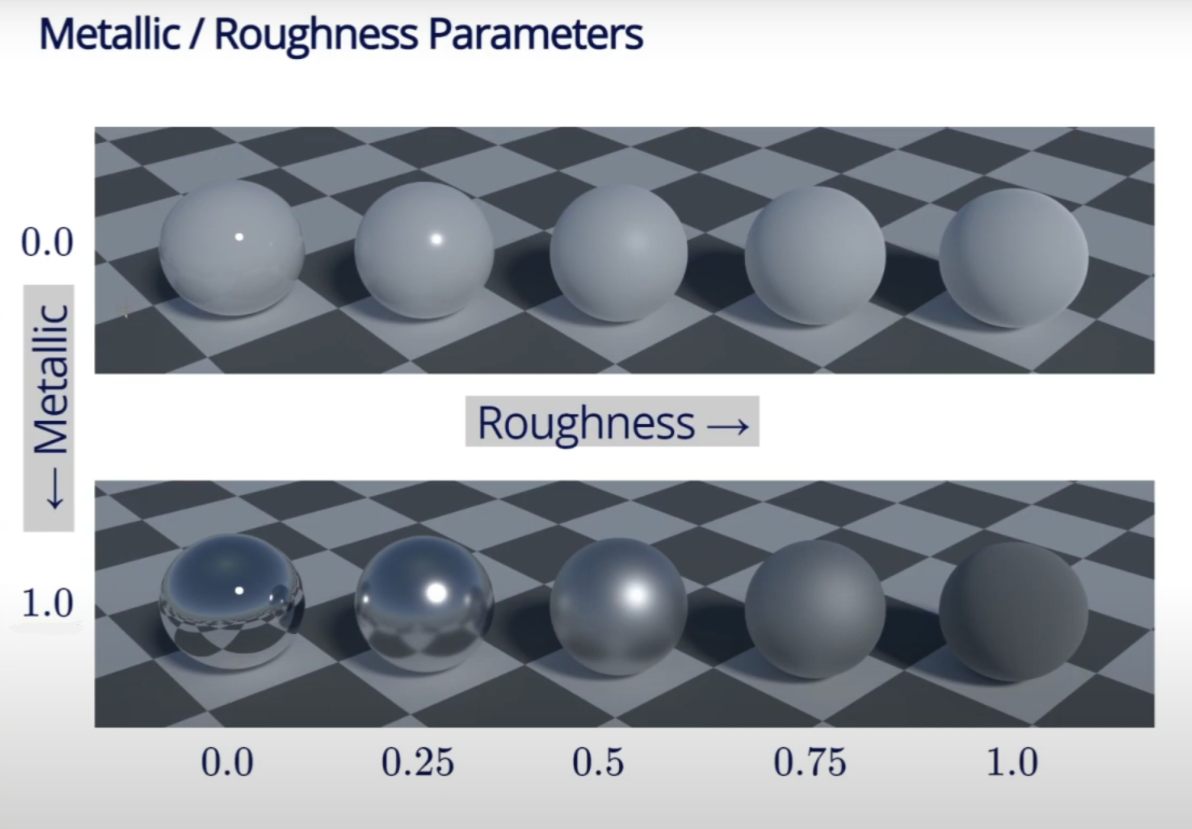
\includegraphics[scale=0.4]{Pictures/rough-metal.png}
  \caption{Металево-шорсткий підхід}
  \label{fig:RM}
\end{figure}

\par
Хоча модель Disney дозволяє використовувати дробові значення па\-ра\-мет\-ра \textit{metallic} (наприклад, $0.5$), фізично це не має сенсу, оскільки матеріал не може 
одночасно бути і металом, і діелектриком. Проте у практичних випадках, особливо при використанні текстур з обмеженою роздільною здатністю, у межах одного 
пікселя може міститися інформація про кілька матеріалів. У таких ситуаціях дробові значення \textit{metallic} інтерпретуються як середнє значення між різними типами 
матеріалів.

\par
Ще одним важливим параметром у моделі є \textbf{базовий колір} (\textit{base color}) рис. (\ref{fig:BC}). Це вектор з трьох компонентів (RGB), 
який відіграє різну роль за\-леж\-но від типу матеріалу.

\begin{itemize}
    \item Для \textbf{діелектриків} (неметалів) цей параметр визначає альбедо ма\-те\-ріа\-лу -- тобто частку світла, яка дифузно відбивається від поверхні. Значення кожної 
    компоненти RGB знаходиться в межах інтервалу $[0;1]$.
    
    \item Для \textbf{металів}, навпаки, \texit{base color} представляє значення коефіцієнта відбиття Френеля при нормальному падінні (Fresnel reflectance), яке 
    характеризує дзеркальну компоненту відбитого світла. Докладний розгляд закону Френеля буде подано у наступному підрозділі.
\end{itemize}

\begin{figure}[h]
  \centering
  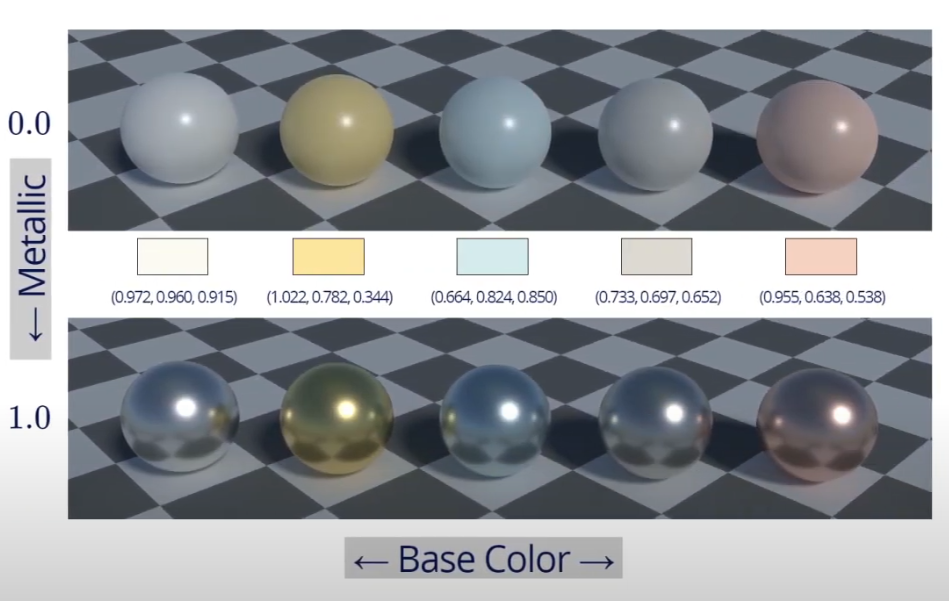
\includegraphics[scale=0.6]{Pictures/BaseColor.png}
  \caption{Базовий колір матеріалів}
  \label{fig:BC}
\end{figure}

Крім того, у моделі передбачено ще один параметр -- \textbf{відбивна здатність} (\textit{reflectance}) рис. (\ref{fig:Specular}), який застосовується лише для діелектричних матеріалів. 
Він також пов’язаний із законом Френеля, однак для неметалів. Цей параметр визначає інтенсивність дзеркальної компоненти відбиття (specular ref\-lec\-tion), 
притаманної діелектрикам.

На відміну від металів, де дзеркальне відбиття при нормальному падінні світла може досягати майже $100\%$, для діелектриків цей показник значно нижчий -- він 
зазвичай перебуває в межах від 0\% до 16\% залежно від матеріалу та кута падіння, та за для зручності ці межі відображають у відрізок $[0,1]$.

\begin{figure}[h]
  \centering
  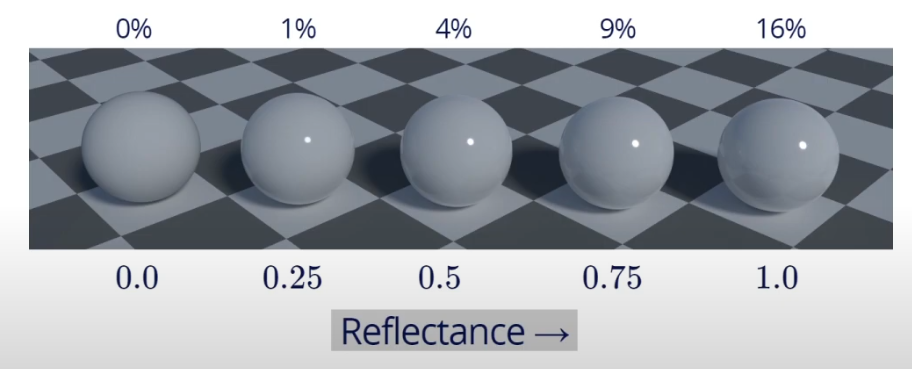
\includegraphics[scale=0.75]{Pictures/Specular.png}
  \caption{Відбивна здатність}
  \label{fig:Specular}
\end{figure}

\par
У рівнянні \ref{eq:RenderingEquation} BRDF виступає у ролі функці $f_r$. Так як BRDF належить до сімейства функцій,
точного вигляду вона немає. В даній квалфікаційній роботі розглядається Cook-Torrance BRDF модель, яка має такий вигляд:
\begin{equation}
\label{eq:BRDF}
f_r(\vec{v},\vec{l}) = \frac{\rho_d}{\pi} + \frac{\mathbf{F}(\vec{v},\vec{h})\cdot\mathbf{D}(\vec{h})\cdot\mathbf{G}(\vec{l},\vec{v})}{4 \cdot\langle \vec{n}, \vec{l}\rangle \cdot\langle \vec{n}, \vec{v}\rangle},
\end{equation}
де, $\vec{v}$ -- це вектор спостереження, тобто вектор у напрямку ока, $\vec{l}$ напрямок промення світла, $\vec{h}$ напівнапрямленний вектор, $\vec{n}$ нормаль поверхні та $\rho_d$ деяка константа.
Тут перший доданок виступає у ролі $f_d$, а другий у ролі $f_s$ рівності \ref{eq:BRDF_DS}. Окрім того, $\mathbf{F}(\vec{v},\vec{h})$ -- відбиття Френеля, $\mathbf{D}(\vec{h})$ -- функція
розподілу нормалей та $\mathbf{G}(\vec{l},\vec{v})$ -- геометричний фактор.

\subsection{Ефект Френеля}
 \setcounter{equation}{0}
 \setcounter{theorem}{0}

Один із ключових етапів побудови фізично коректної моделі відбиття світла полягає у врахуванні \textit{ефекту Френеля}, який описує залежність коефіцієнта 
відбиття від кута падіння світла та показників заломлення матеріалів на межі поділу середовищ.

\par
Ефект Френеля легко можна спостерігати в реальному житті. Наприклад, на рис.\ref{fig:FresnelLake} зображено озеро з абсолютно рівною поверхнею води; у нижній час\-ти\-ні чітко видно дно. 
Натомість у верхній частині видно лише відбиття. Така різниця пояснюється тим, що співвідношення між переданим і відбитим світ\-лом не є сталим: воно змінюється 
залежно від кута падіння променя та оп\-тич\-них властивостей (показників заломлення) матеріалів.

Коли ми дивимося у воду під прямим кутом, лише незначна частина світла відбивається, решта проходить крізь поверхню води, і ми бачимо дно. Проте зі збільшенням кута
 (наближенням до дотичного спостереження), частка відбитого світла зростає, а частка переданого -- зменшується. Тобто при малих кутах падіння спостерігається в основному 
 пропускання, а при великих -- відбиття.

 \begin{figure}[h]
  \centering
  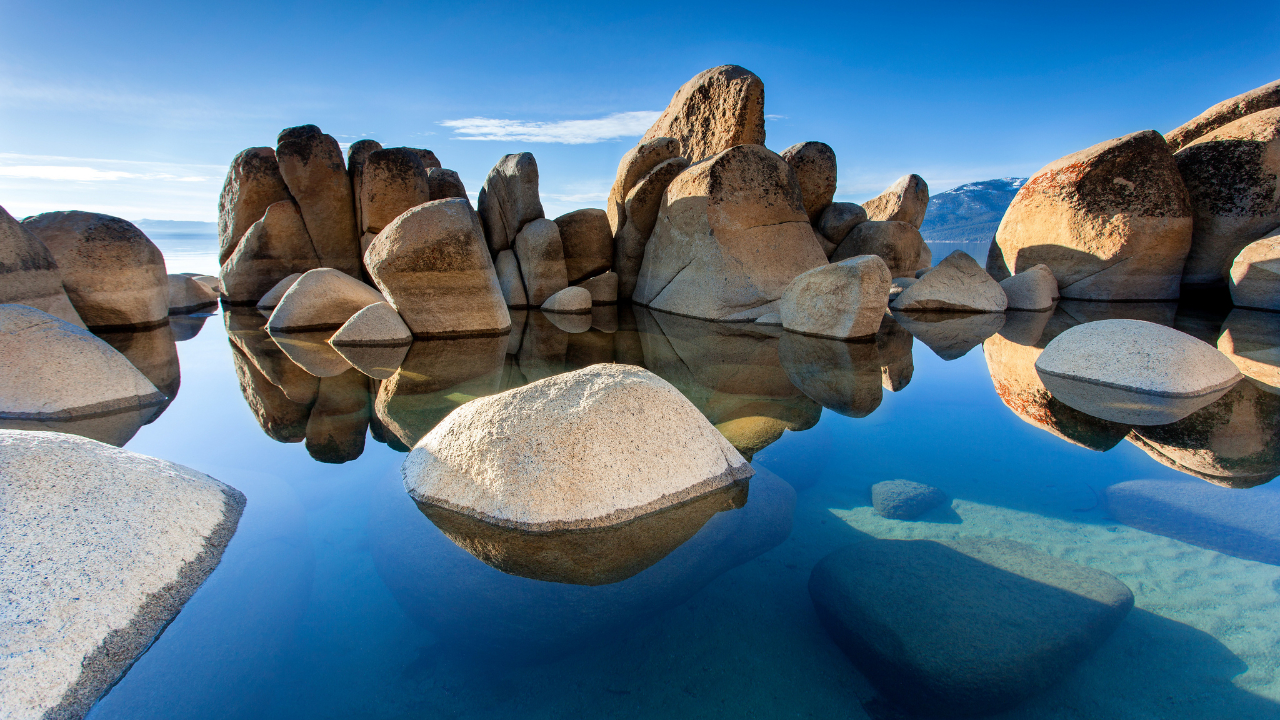
\includegraphics[scale=0.25]{Pictures/fresnelLake.jpg}
  \caption{Ефект Френеля в реальному житті}
  \label{fig:FresnelLake}
\end{figure}

\newpage
На рис. \ref{fig:Snells} зображено типову ситуацію взаємодії світла з поверхнею на межі двох середовищ. У випадку басейну це межа повітря 
(з показником заломлення $\eta_1$) і води (з більшим показником заломлення $\eta_2$). Кут падіння $\theta_1$ визначається відносно нормалі до поверхні. Закон 
відбиття стверджує, що кут між нормаллю та відбитим променем дорівнює $\theta_1$. Для заломленого (переданого) променя кут $\theta_2$ є меншим, оскільки світло 
переходить із менш густого середовища у густіше (тобто промені заломлюються у бік нормалі).

Цей зв’язок описується законом Снеліуса:
\begin{equation*}
    \eta_1 \sin \theta_1 = \eta_2 \sin \theta_2,
\end{equation*}
де $\eta_1$ та $\eta_2$ -- показники заломлення відповідних середовищ, $\theta_1$ -- кут падіння, а $\theta_2$ -- кут заломлення.


 \begin{figure}[h]
  \centering
  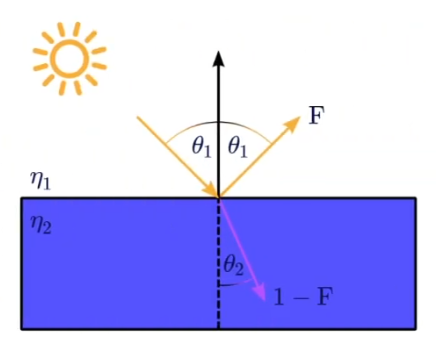
\includegraphics[scale=0.75]{Pictures/Snells.png}
  \caption{Заломлення світла}
  \label{fig:Snells}
\end{figure}

Знаючи $\eta_1$, $\eta_2$ та $\theta_1$, ми можемо обчислити $\theta_2$ і, у подальшому, розрахувати частку відбитого світла за допомогою рівнянь Френеля:
\begin{equation*}
F_{para} = \frac{\eta_2\cos\theta_1 - \eta_1\cos\theta_2}{\eta_2\cos\theta_1 + \eta_1\cos\theta_2};
\end{equation*}
\begin{equation*}
F_{pere} = \frac{\eta_2\cos\theta_2 - \eta_1\cos\theta_1}{\eta_2\cos\theta_2 + \eta_1\cos\theta_1};
\end{equation*}
\begin{equation}
\label{eq:fresnel}
F = \frac{1}{2}(F_{para} + F_{pere}).\quad
\end{equation}

Частка переданого світла визначається як:
\begin{equation*}
    T = 1 - R,
\end{equation*}
де $R$ -- коефіцієнт відбиття, який залежить від поляризації світла, кута падіння та оптичних властивостей матеріалів.
\paragraph{Відбиття Френеля для діелектриків та металів.}

\par 
Світлові фотони при взаємодії з поверхнею можуть бути відбитими із певними йомовірностями, які напряму залежать від кута падіння. Для діе\-ле\-кт\-ри\-ків, відбита частина світла розсіюється мікрофасетками поверхні, що мак\-ро\-ско\-піч\-но формує дзеркальну складову відбиття. Передана частина зазнає внут\-ріш\-ніх 
 розсіянь, частково поглинається і випромінюється у випадкових напрямках. Це створює дифузну складову.
Чим більше світла відбивається на поверхні, тим менше його проникає всередину, а отже, дифузна складова стає слабшою. Оскільки ймовірність поглинання світла 
залежить від довжини хвилі, то дифузна частина є кольоровою. Натомість дзеркальна складова зазвичай є некольоровою для діелектриків.


\par
Для металів ситуація інакша: передана частина повністю поглинається, тому дифузна складова відсутня. Натомість дзеркальна складова є кольоровою, оскільки залежить
 від довжини хвилі. Це пояснює, чому метали мають ха\-рак\-тер\-не забарвлення у дзеркальних відбиттях.

 \par
Для перпендикулярного падіння ($\theta_1 = 0^\circ$), рівняння Френеля значно спрощуються. Якщо припустити, що $\eta_1 = 1$ (повітря або вакуум), а $\eta_2 = 1.5$ 
(наприклад, скло), то за формулою \ref{eq:fresnel} можна обчислити значення $F_0 \approx 0.04$, тобто $4\%$ світла буде відбито, а 96\% -- пропущено.

\begin{equation*}
    F_0 = \left( \frac{\eta_2 - \eta_1}{\eta_2 + \eta_1} \right)^2.
\end{equation*}

\par 
У мікрофасетній моделі поверхня складається з великої кількості кри\-хіт\-них ідеально плоских дзеркал. Через це для розрахунку відбиття Френеля ми використовуємо не кут між 
вхідним променем та нормаллю поверхні, а кут між напрямком огляду (або світла) і вектором півшляху (halfway vector). У данному випадку
вектор півшляху використовується як нормаль мікрофасеток через те, що нас цікавить частина світла яка відбивається у напрямок спостерігача:

\begin{equation}
    \cos \theta = \langle\vec{v}, \vec{h}\rangle.
\end{equation}

Тому саме цей кут $\theta$ використовується у рівняннях Френеля в мікрофасетній BRDF-моделі, запропонованій Куком і Торренсом (Cook \& Torrance, 1982) \cite{cook1982reflectance}, та
ефект Френеля обчислюється наступним чином:
\begin{equation}
  F_{Cook-Torrance}(\vec{v},\vec{h}) = \frac{1}{2}(\frac{g - c}{g + c})^2(1 + (\frac{c(g+c)-1}{c(g-c)+1})^2),
\end{equation}
де $c = \langle\vec{v},\vec{h}\rangle$ та $g = \sqrt{\eta_2^2+c^2-1}$.
Незважаючи на відсутність тригонометричних функцій, ці обчислення є дорогими. Щоб зменшити обчислювальні витрати, часто використовують \textit{апроксимацію 
Шліка (aнгл. Schlick's approximation)}:

\begin{equation}
    F_{Schlick}(\theta) = F_0 + (1 - F_0)(1 - \cos \theta)^5.
\end{equation}

Ця формула дозволяє швидко наближати поведінку функції Френеля без втрати надто великої точності.
 Як показано на рис. \ref{fig:Schlick}, при $\theta = 0^\circ$ вона точно дає $F = F_0$, а при $\theta = 90^\circ$ -- $F = 1$. 
 У проміжних кутах апроксимація лише незначно відхиляється від точного розв’язку.
 \begin{figure}[h]
  \centering
  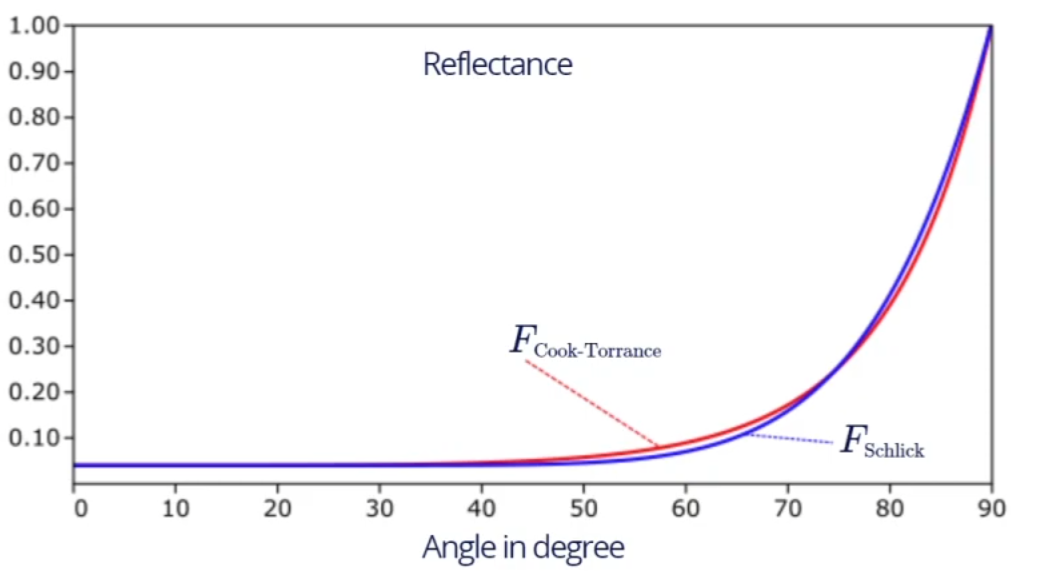
\includegraphics[scale=0.55]{Pictures/Shlick.png}
  \caption{Порівняння апроксимацію Шліка}
  \label{fig:Schlick}
\end{figure}

Цей підхід широко використовується у реальному часі (наприклад, у PBR-шейдерах), забезпечуючи добрий баланс між точністю і швидкодією.

\subsection{Функція розподілу нормалей}\\

\par
Як вже зазначалося раніше, поверхня фізичного матеріалу має мікроскопічну шорсткість, яка складається з безлічі мікрофасетів із власними мікронормалями. 
Ця мікроструктура відіграє ключову роль у формуванні зовнішнього вигляду поверхні під час взаємодії зі світлом.

Розподіл таких мікронормалей описується за допомогою функції розподілу нормалей (NDF, \textit{Normal Distribution Function}). Вона є складовою частиною 
двонапрямної функції розподілу відбиття, яка визначає, як світло від\-би\-ва\-єть\-ся з поверхні y 
заданому напрямку.

BRDF формалізує кількість енергії, що відбивається від поверхні в напрямку спостерігача від одного променя вхідного світла. Вона є зваженою величиною, оскільки 
враховує NDF, яка насправді є функцією розподілу ймовірностей (PDF, \textit{Probability Distribution Function}) для напрямків мікронормалей.

У випадку ідеально гладкої, полірованої поверхні всі мікрофасети орієнтовані в одному напрямку -- відповідно до макроскопічної нормалі поверхні. Натомість 
при більш шорсткій поверхні орієнтації мікрофасетів статистично розподілені навколо цієї нормалі. Відповідно, відбиття світла також розсіюється навколо ідеального
 дзеркального напрямку. Із зростанням шорсткості поверхні ступінь цього розсіювання збільшується рис. (\ref{fig:NDF}).

  \begin{figure}[h]
  \centering
  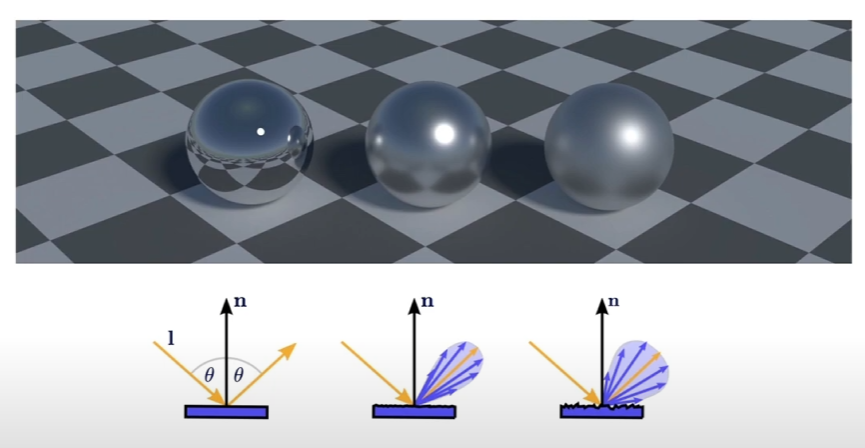
\includegraphics[scale=1]{Pictures/NDF.png}
  \caption{Вплив функції розподілу нормалей}
  \label{fig:NDF}
\end{figure}

Таким чином, функція розподілу нормалей NDF визначає, наскільки вірогідною є наявність мікрофасета певної орієнтації в даній точці поверхні. Ця ймовірність 
безпосередньо впливає на вигляд відбитого світла, а отже -- і на візуальне сприйняття матеріалу.
\par 
  У моделі Cook-Torrance, NDF розраховується за формулою:
\begin{equation}
  D_{GGX}(\vec{h})=\frac{\alpha^2}{\pi(\langle\vec{n},\vec{h}\rangle^2(\alpha^2-1)+1)^2},
\end{equation}
де $\alpha = r_p^2$, а $r_p$ -- шорсткість матеріалу та приймає значення на відрізку $[0,1]$.

\subsection{Геометричний фактор}\\

\par
Останнім елементом мікрофасетної моделі є геометричний фактор, який враховує ефекти затінення (\textit{shadowing}) та перекриття (\textit{masking}) 
мікрофасетів. Ці ефекти виникають залежно від напрямку падіння світла та напрямку огляду спостерігача.

У роботі Кука і Торренса, передбачається, що мікрофасети мають форму літери V. 
На основі цієї моделі було виведено геометричний термін, який описує ймовірність того, що світло буде заблоковане іншими мікрофасетами 
або не зможе відбитися в напрямку спостерігача, обчислюється він наступним чином:
\begin{equation*}
  G_{Cook-Torrance}(\vec{l},\vec{v}) = min(1, \frac{2\langle\vec{n},\vec{h}\rangle\langle\vec{n},\vec{v}\rangle}
  {\langle\vec{v},\vec{h}\rangle},
  \frac{2\langle\vec{n},\vec{h}\rangle\langle\vec{n},\vec{l}\rangle}
  {\langle\vec{v},\vec{h}\rangle}).
\end{equation*}

Залежно від конфігурації, можливі три випадки: відсутність перешкод, \linebreak ефект перекриття при поглядових кутах під ковзаючим кутом, 
або затінення при падінні світла під аналогічним кутом (див. рис. \ref{fig:GeometryTerm}).Для нульового значення шорсткості (ідеально гладка поверхня) геометричний фактор дорівнює 1, 
тобто не впливає на результат. Зі збільшенням шорсткості значення геометричного фактору зменшується, 
що відповідає фізично очікуваному ефекту -- зростанню ймовірності перекриття і затінення мікрофасетів.

\begin{figure}[h]
  \centering
  \hspace*{-1.7cm} % або -0.1cm, -2mm тощо
  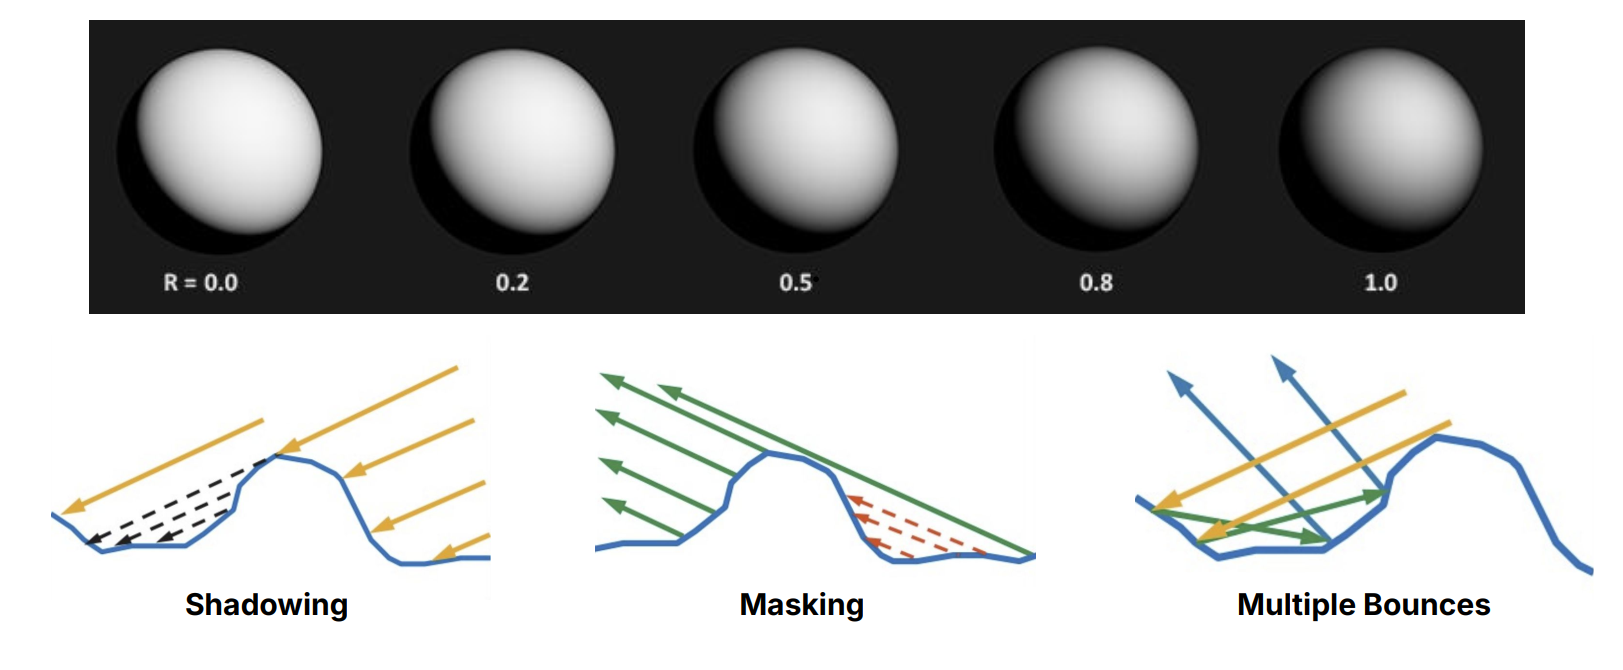
\includegraphics[scale=0.65]{Pictures/GeometryTerm.png}
  \caption{Вплив геометричного фактору}
  \label{fig:GeometryTerm}
\end{figure}



Іншу відому модель геометричного фактору запропонував Б.~Дж.~Сміт\linebreak (B.~J.~Smith) у 1967 році. 
У ній геометричний фактор обчислюється як добуток двох однакових функцій $G_1$, які розраховуються окремо для напрямку світла та напрямку огляду:

\[
G(l, v) = G_1(l) \cdot G_1(v).
\]

За функцію $G_1$ було обрано:
\begin{equation*}
  G(\vec{v}) = \frac{\sqrt{2}}{\sqrt{1 + \frac{\alpha(1-\langle\vec{n},\vec{v}\rangle)}{\langle\vec{n},\vec{v}\rangle}}}.
\end{equation*}
Таким чином, остаточне аналітичне представлення геометричного фактору, що враховує вплив мікроструктури поверхні на явища екранування та за\-ті\-нен\-ня, набуває наступного вигляду:

\begin{equation}
  \label{eq:GT}
G = \frac{2}{\sqrt{1 + \frac{\alpha(1-\langle\vec{n},\vec{v}\rangle)}{\langle\vec{n},\vec{v}\rangle}}
\sqrt{1 + \frac{\alpha(1-\langle\vec{n},\vec{l}\rangle)}{\langle\vec{n},\vec{l}\rangle}}}.
\end{equation}

Цей вираз є кульмінацією теоретичного узагальнення мікрофасетної геометрії, що водночас 
враховує складні взаємодії світлового потоку з текстурною нерівністю реальних поверхонь. Його 
застосування забезпечує фізично коректне моделювання поведінки світла на мікроскопічному рівні, що 
є критично важливим для створення фотореалістичних комп’ютерних зображень.

\par Такий підхід дозволяє точно моделювати як дифузні, так і дзеркальні відбиття, залежно від
оптичних характеристик матеріалу, зокрема показника заломлення, ступеня шорсткості та кута падіння 
світла. Завдяки цьому, система освітлення здатна відтворювати складну взаємодію світла з матеріалом -- 
від блискучих металів до матових діелектриків -- з урахуванням енергозбереження та фізичної правдоподібності.

\par У практичній реалізації мікрофасетної моделі критичним є вибір функції розподілу нормалей 
поверхні (NDF), таких як GGX або Beckmann, які визначають імовірнісний розподіл мікрофасеток по орієнтаціях. 
Це, в поєднанні з геометричними термінами самозатінення (G) та френелівськими коефіцієнтами (F), утворює 
повноцінну BRDF-модель (наприклад, Кука-Торренса), що дозволяє інтегрувати фізику світлових явищ 
у рендерінг-алгоритми сучасних графічних рушіїв.

\par Саме через ці характеристики мікрофасетна модель виступає основою у більшості сучасних 
технік фізично коректного рендерингу (PBR) і є фундаментом для багатьох подальших удосконалень, 
включаючи імплементацію попередньо обчислених таблиць (LUT), вибір за значимістю (англ. importance sampling), а також 
застосування моделей освітлення на основі оточення (IBL), що в сукупності дозволяє досягати високого 
візуального реалізму при збереженні продуктивності.

% ***************************************************************************
 \chapter{ЧИСЛОВІ ЕКСПЕРИМЕНТИ}
У цьому розділі проведено числові експерименти з метою візуальної та функціональної перевірки реалізованих фізично коректних моделей рендерингу

\section{Середовище розробки та обладнання}
\setcounter{equation}{0}
\setcounter{theorem}{0}    

Усі числові експерименти були виконані на ноутбуці Asus ROG Strix G15. Характеристики цього пристрою наведені нижче:

\begin{itemize}
    \item \emph{GPU:} LAPTOP NVIDIA RTX 3060 з 6GB відеопам'яті;
    \item \emph{CPU:} AMD Ryzen 7 6800H, 8 ядер, 16 потоків, з тактовою частотою до 4.7GHz;
    \item \emph{Оперативна пам'ять:} 16GB DDR5;
    \item \emph{SSD:} Kingston KC3000 з швидкістю читання/запису до 7GB/сек.
\end{itemize}

\subsection{Середовище розробки}

Для розробки, налагодження та візуалізації результатів було використано такі інструменти:

\begin{itemize}
    \item \emph{Visual Studio Community 2022} -- основне середовище розробки C++ та HLSL, з підтримкою проєктів на основі DirectX 11/12.
    
    \item \emph{RenderDoc} -- потужний GPU-дебаггер та фрейм-граббер, що дозволив проводити глибокий аналіз рендеринг-пайплайну, діагностувати помилки та профілювати продуктивність шейдерів.
    
    \item \emph{Microsoft PIX} -- інструмент для глибокого профілювання GPU та CPU, з можливістю детального перегляду часу виконання кожного кадру та виявлення вузьких місць у продуктивності.
    
    \item \emph{Gpu-Z} -- утиліта для моніторингу завантаження GPU, частоти та температури під час виконання сцени рендерингу.
    
    \item \emph{Visual Studio Graphics Analyzer} -- вбудований профайлер графіки у складі Visual Studio, використовувався для перевірки коректності відправки ресурсів у GPU.
\end{itemize}

\subsection{Використані бібліотеки}

У реалізації рендерера були використані численні зовнішні бібліотеки для прискорення розробки, обробки ресурсів, імпорту моделей, UI-компонентів тощо:

\begin{itemize}
    \item \emph{DirectX 11 API} -- основна графічна API для реалізації низькорівневого рендерингу та управління GPU-ресурсами;
    
    \item \emph{DirectXMath} -- векторна та матрична бібліотека, оптимізована під SIMD-операції, яка використовувалася для математичних обчислень на CPU;
    
    \item \emph{DirectXTex} -- бібліотека для обробки текстур, включно з генерацією MIP-рівнів, стисненням формату BCn та конвертацією HDR/PNG/TGA;
    
    \item \emph{Assimp (Open Asset Import Library)} -- кросплатформенна бібліотека для імпорту 3D-моделей у форматах .fbx, .obj, .dae та інших;
    
    \item \emph{Dear ImGui} -- GUI-фреймворк для створення вікон, слайдерів, графіків та інших відладочних елементів у реальному часі;
    
    \item \emph{stb\_image та stb\_image\_write} -- загальновідомі заголовкові бібліотеки для завантаження та збереження зображень у форматах .png, .jpg, .hdr;
    
    \item \emph{d3dx12/d3d11helper} -- набір допоміжних функцій і утиліт для спрощення роботи з ресурсами Direct3D (створення буферів, SRV/RTV тощо);
    
    \item \emph{WinPixEventRuntime} -- для маркування GPU-подій у рендерері та полегшення аналізу у PIX;
    
    \item \emph{tinyobjloader} -- легка бібліотека для прямого завантаження .obj-файлів у проєкті без повного стеку Assimp.
\end{itemize}

\section{Особливості роботи з DirectX 11}

За інтерфейс програмування застосунків(API) було використано
\texit{DirectX 11}, адже він є сумісним з операційною системою(ОС) Windows, та є відносно простим у використані, на відміну від його нащадка \textit{DirectX 12}.Важливою частиною розробки онлайн фізично обрґрунтованого симулювання освітлення є оптимізація, адже чим оптимінізованішим буде \textit{графічний рушій} -- програмне забезпечення, яке займається рендерингом сцен, тим краща модель симуляції освітлення зможе бути використана для наближення сцени до зображень, які ми бачимо оком.

\subsection{Текстурування та MIP-текстурування}

Однією з ключових тех\-нік оптимізації відображення текстур у рендерингу є \textbf{MIP-текстурування}. Це метод, який передбачає зберігання кількох копій однієї і тієї ж текстури з різним рівнем деталізації, як показано на рис.~\ref{fig:Mip}.

\begin{figure}[h]
  \centering
  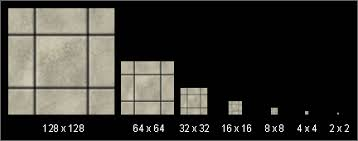
\includegraphics[scale=0.75]{Pictures/images.jpeg}
  \caption{Схематичне зображення MIP-текстурування}
  \label{fig:Mip}
\end{figure}

Зазвичай розміри текстур задані як степені двійки, наприклад, $$1024 \times 1024 = 2^{10} \times 2^{10}.$$ Це дозволяє легко створювати кожен наступний рівень MIP-текстури з деталізацією, зменшеною вдвічі порівняно з попереднім, тобто:
\[
\text{MIP}_{n+1} = \frac{\text{MIP}_n}{2}.
\]

Таким чином, кожен рівень зменшує площу текстури у чотири рази, а сумарне споживання пам’яті усіх рівнів MIP-текстур становить приблизно на $33\%$ більше, ніж для оригінальної текстури. Це випливає з геометричної прогресії площ:
\[
\sum_{n=1}^{\infty} \left(\frac{1}{4^n}\right) = \frac{1}{3}.
\]

Переваги використання MIP-текстурування полягають не лише в зменшенні навантаження на відеопам’ять та обчислювальні ресурси, але й у покращенні візуальної якості зображення. Зокрема, при рендерингу об’єктів, розташованих на значній відстані від камери, немає необхідності застосовувати пов\-но\-роз\-мір\-ну текстуру, адже спостерігач все одно не зможе розрізнити дрібні деталі. У таких випадках використовується менш детальна копія текстури, що знижує кількість вибірок у піксельному шейдері та підвищує продуктивність.

Окрім оптимізації, MIP-текстурування відіграє важливу роль у боротьбі з \textbf{муаровим ефектом}~(рис.~\ref{fig:Muar}) -- артефактом, що виникає внаслідок накладання високочастотної текстури на об’єкти, які займають невелику кількість пікселів на екрані. У таких випадках без MIP-текстурування може спостерігатися некоректна інтерполяція пікселів під час руху камери, що призводить до неприємного візуального мерехтіння.

\begin{figure}[h]
  \centering
  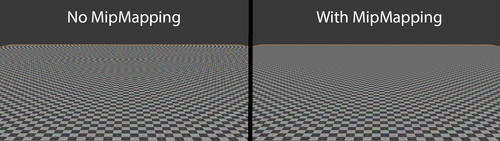
\includegraphics[scale=0.8]{Pictures/Mipmap_Aliasing_Comparison.png}
  \caption{Порівняння зображення з використанням та без використання MIP-текстурування}
  \label{fig:Muar}
\end{figure}
\newpage
\subsection{Рівень деталізації (Level of Detail, LOD)} \mbox{}\
\par Техніка рівня деталізації (LOD) полягає в динамічному виборі гео\-мет\-рич\-ної складності об'єкта залежно від відстані до камери. Ідея подібна до MIP-текстурування (рис.~\ref{fig:Mip}), але застосовується до геометрії (рис.~\ref{fig:LOD}), а не до текстур. У цьому підході для кожного об'єкта готується кілька версій моделі з різ\-ним числом полігонів -- від максимально деталізованої до значно спрощеної.

\begin{figure}[h]
  \centering
  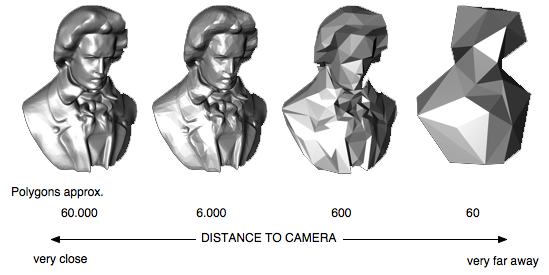
\includegraphics[scale=0.75]{Pictures/lod.png}
  \caption{Різні рівні деталізації}
  \label{fig:LOD}
\end{figure}

\par Під час рендерингу рушій або GPU автоматично вибирає відповідний рівень деталізації залежно від відстані до об'єкта чи його розміру на екрані. Наприклад, якщо об'єкт розташований далеко від камери, він займає менше пік\-се\-лів, і використання повністю деталізованої моделі стає недоцільним з точ\-ки зору продуктивності. Замість цього обирається менш складна геометрична версія, яка майже не відрізняється візуально на такій відстані, але значно знижує навантаження на GPU.

\par Подібно до MIP-текстурування, яке використовує різні версії текстури для зменшення артефактів та оптимізації пам’яті, LOD дозволяє досягти балансу між візуальною якістю та продуктивністю, зменшуючи кількість обчислень, необхідних для віддалених об’єктів. Це критично важливо у великих відкритих сценах, де на екрані одночасно може бути присутня велика кількість об’єктів.

\par У деяких випадках використовується так звана безперервна LOD (Con\-ti\-nuous LOD), де геометрія плавно змінюється замість різкого перемикання між рівнями, що дозволяє уникнути візуальних артефактів у вигляді ``помітного стрибка`` при зміні моделі.

\subsection{Відкладене освітлення та затінювання (Deferred Shading)} \mbox{}\
\par Однією з найефективніших технік оптимізації рендерингу в сучасних графічних рушіях є відкладене освітлення та затінювання (Deferred Shading). Ос\-нов\-на ідея полягає в розділенні етапів рендерингу сцени на дві фази: збір геометричної інформації та обрахунок освітлення.

\par На першому етапі виконується рендеринг геометрії сцени у так звані G-буфери (geometry buffers) (рис.\ref{fig:G}) -- набір текстур, що зберігають усю необхідну інформацію про пікселі:
\begin{itemize}
\item глибину (depth buffer, z-buffer);
\item нормалі поверхонь (normal buffer);
\item базовий колір (albedo);
\item властивості матеріалів, такі як шорсткість і металічність (roughness-metalness buffer).
\end{itemize}

\begin{figure}[h]
  \centering
  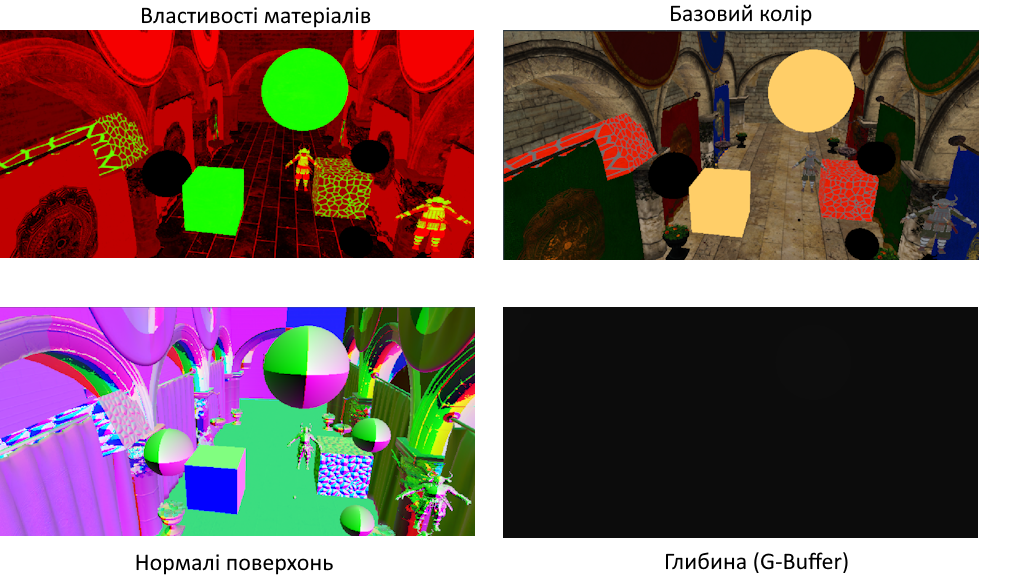
\includegraphics[scale=0.75]{Pictures/G-buffer.png}
  \caption{G-буфери}
  \label{fig:G}
\end{figure}


\par Після цього, на другому етапі, система виконує обчислення освітлення, використовуючи інформацію з G-буферів лише для пікселів, що дійсно потрапили у фінальний кадр. Таким чином, обчислення освітлення відбувається лише для видимих фрагментів, що значно зменшує кількість непотрібних операцій порівняно з прямим (forward) рендерингом, де освітлення розраховується для всіх об'єктів незалежно від того, чи видно їх на екрані.

\par Основною перевагою відкладеного затінювання є його масштабованість при великій кількості джерел світла, оскільки світло розраховується по\-ст\-фак\-тум у екранізованому просторі, а не для кожного пікселя кожного об’єкта окремо. Це дозволяє значно підвищити продуктивність у складних сценах із ба\-гать\-ма джерелами світла.

\par Водночас, варто враховувати і недоліки: зокрема, складність підтримки прозорих об’єктів, високі вимоги до пам’яті GPU через велику кількість G-буферів, а також обмеження при використанні MSAA (Multisample Anti-Alia\-sing).

\section{Результати числових експериментів}

\par У цьому підрозділі наведено результати реалізації основних теоретичних положень, розглянутих у попередніх розділах, зокрема методів фізично коректного рендерингу (PBR), мік\-ро\-фа\-сет\-ко\-вої BRDF-моделі Кука–Торренса, процедур MIP-мапінгу, організації рівнів деталізації, реалізації відкладеного затінення (deferred shading), а також оптимізаційних технік, що були інтегровані у рендеринг-пайплайн.

\par Перш ніж перейти до поетапного аналізу впливу окремих фізичних параметрів на результуюче зображення, на рис.~\ref{fig:overview} та \ref{fig:close_overview} продемонстровано загальний вигляд сцени, що візуалізує повноцінну реалізацію системи освітлення із урахуванням усіх складових PBR-моделі.

\begin{figure}[h]
\centering
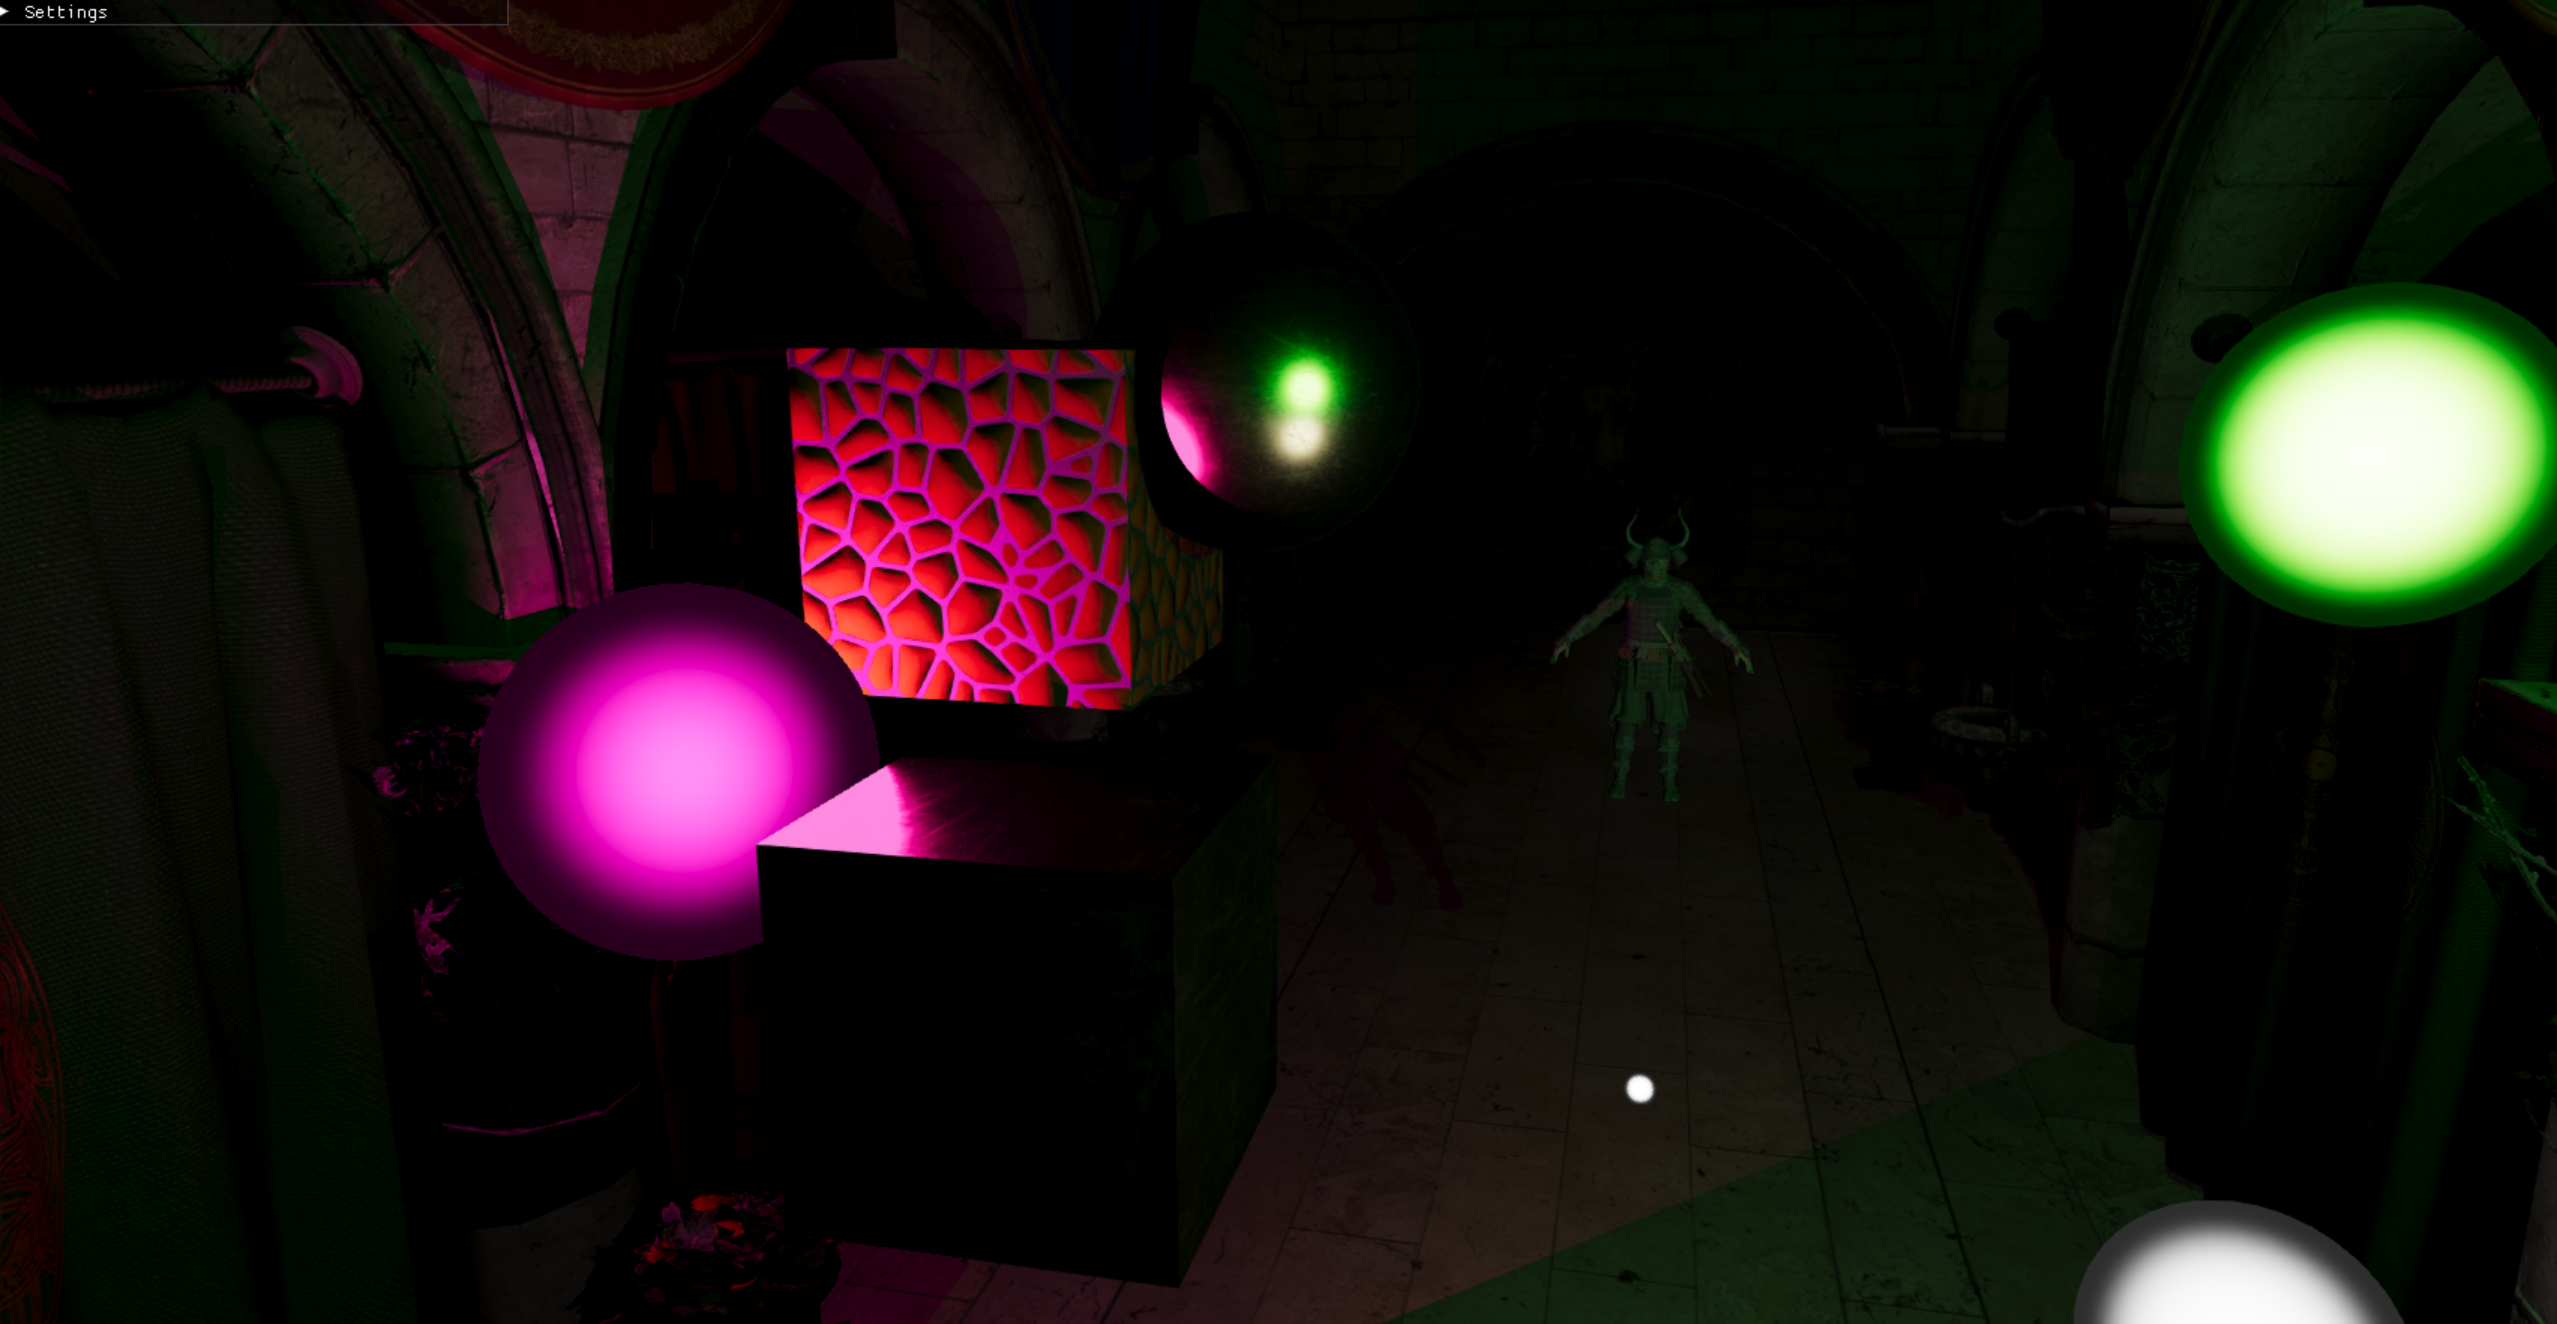
\includegraphics[scale = 0.2125]{Pictures/1.png}
\caption{Загальний вигляд сцени з реалізованою PBR-системою}
\label{fig:overview}
\end{figure}

\begin{figure}[h]
\centering
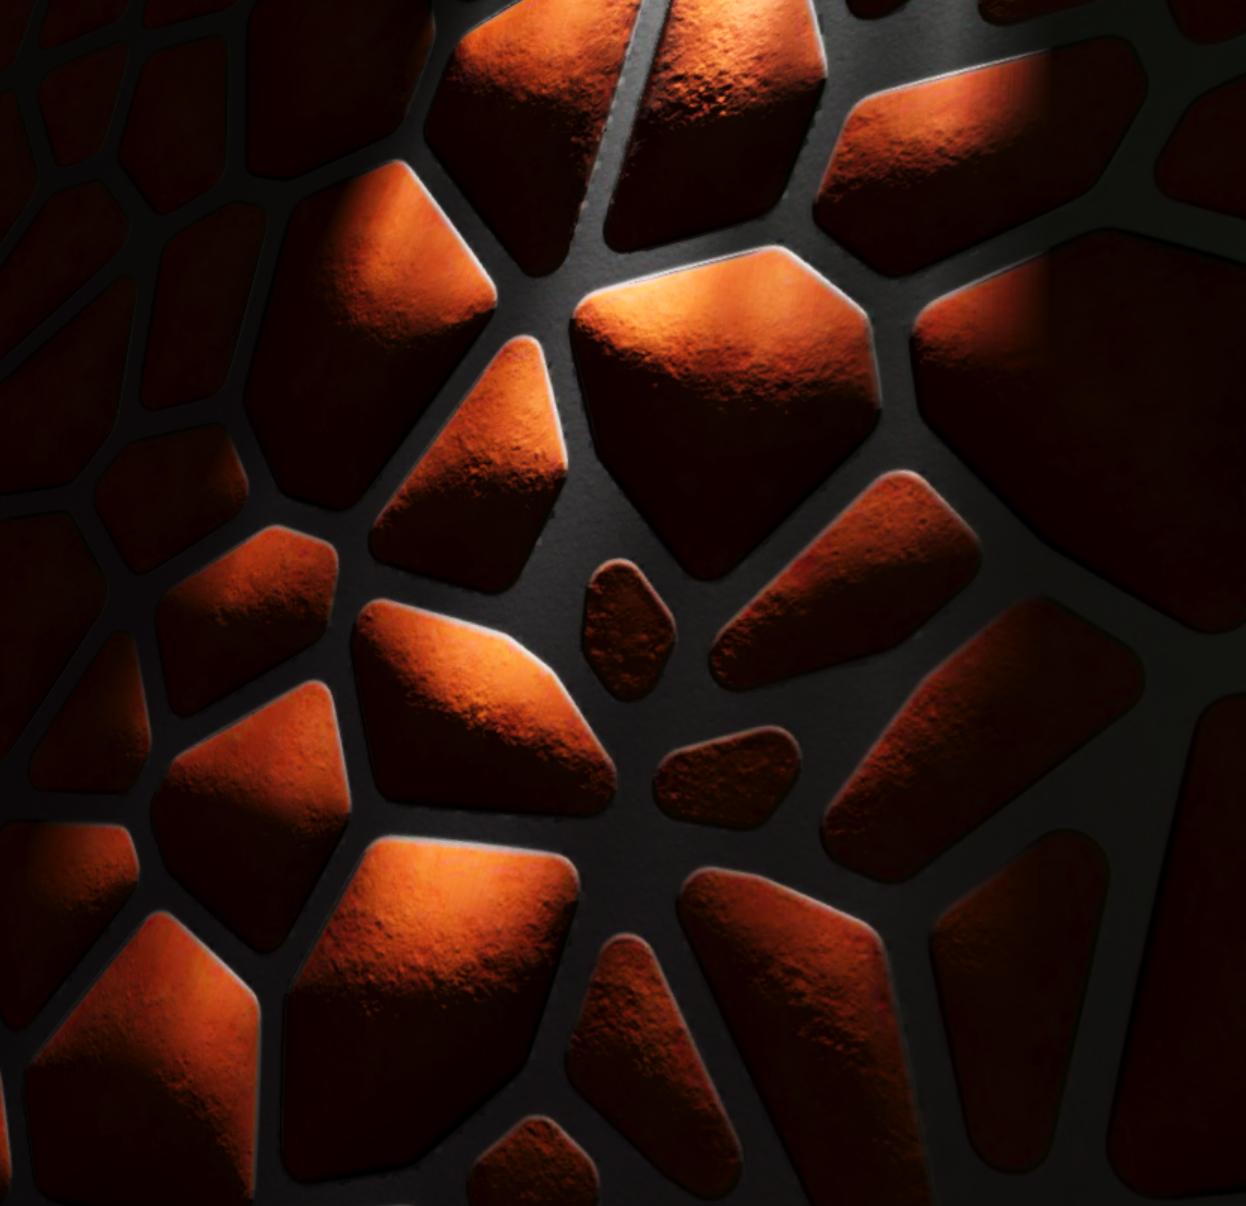
\includegraphics[scale = 0.2125]{Pictures/12.png}
\caption{Фрагмент сцени: вигляд об'єктів крупним планом}
\label{fig:close_overview}
\end{figure}

\par Для демонстрації впливу матеріальних властивостей на вигляд поверхні було проведено серію експериментів із візуалізацією сферичних об’єктів при різних значеннях параметрів металічності ($metalness$) та шорст\-кос\-ті ($roughness$). Зокрема:

\begin{itemize}
\item Металева сфера з $metalness = 1.0$ та $roughness = 0.5$, з просторовими варіаціями параметрів по поверхні -- демонструє роботу мікро\-фа\-сет\-ко\-вої BRDF-моделі.
\item Та ж сфера з високою шорсткістю ($roughness = 0.9$), що зумовлює розмиття дзеркального відбиття.
\item Ідеально гладка металева сфера ($roughness = 0.0$), яка відображає навколишнє середовище з максимальною чіткістю.
\item Діелектрична сфера ($metalness = 0.0$), яка не створює дзеркального відбиття, натомість формує лише дифузне розсіювання світла.
\end{itemize}

\begin{figure}[h]
\centering
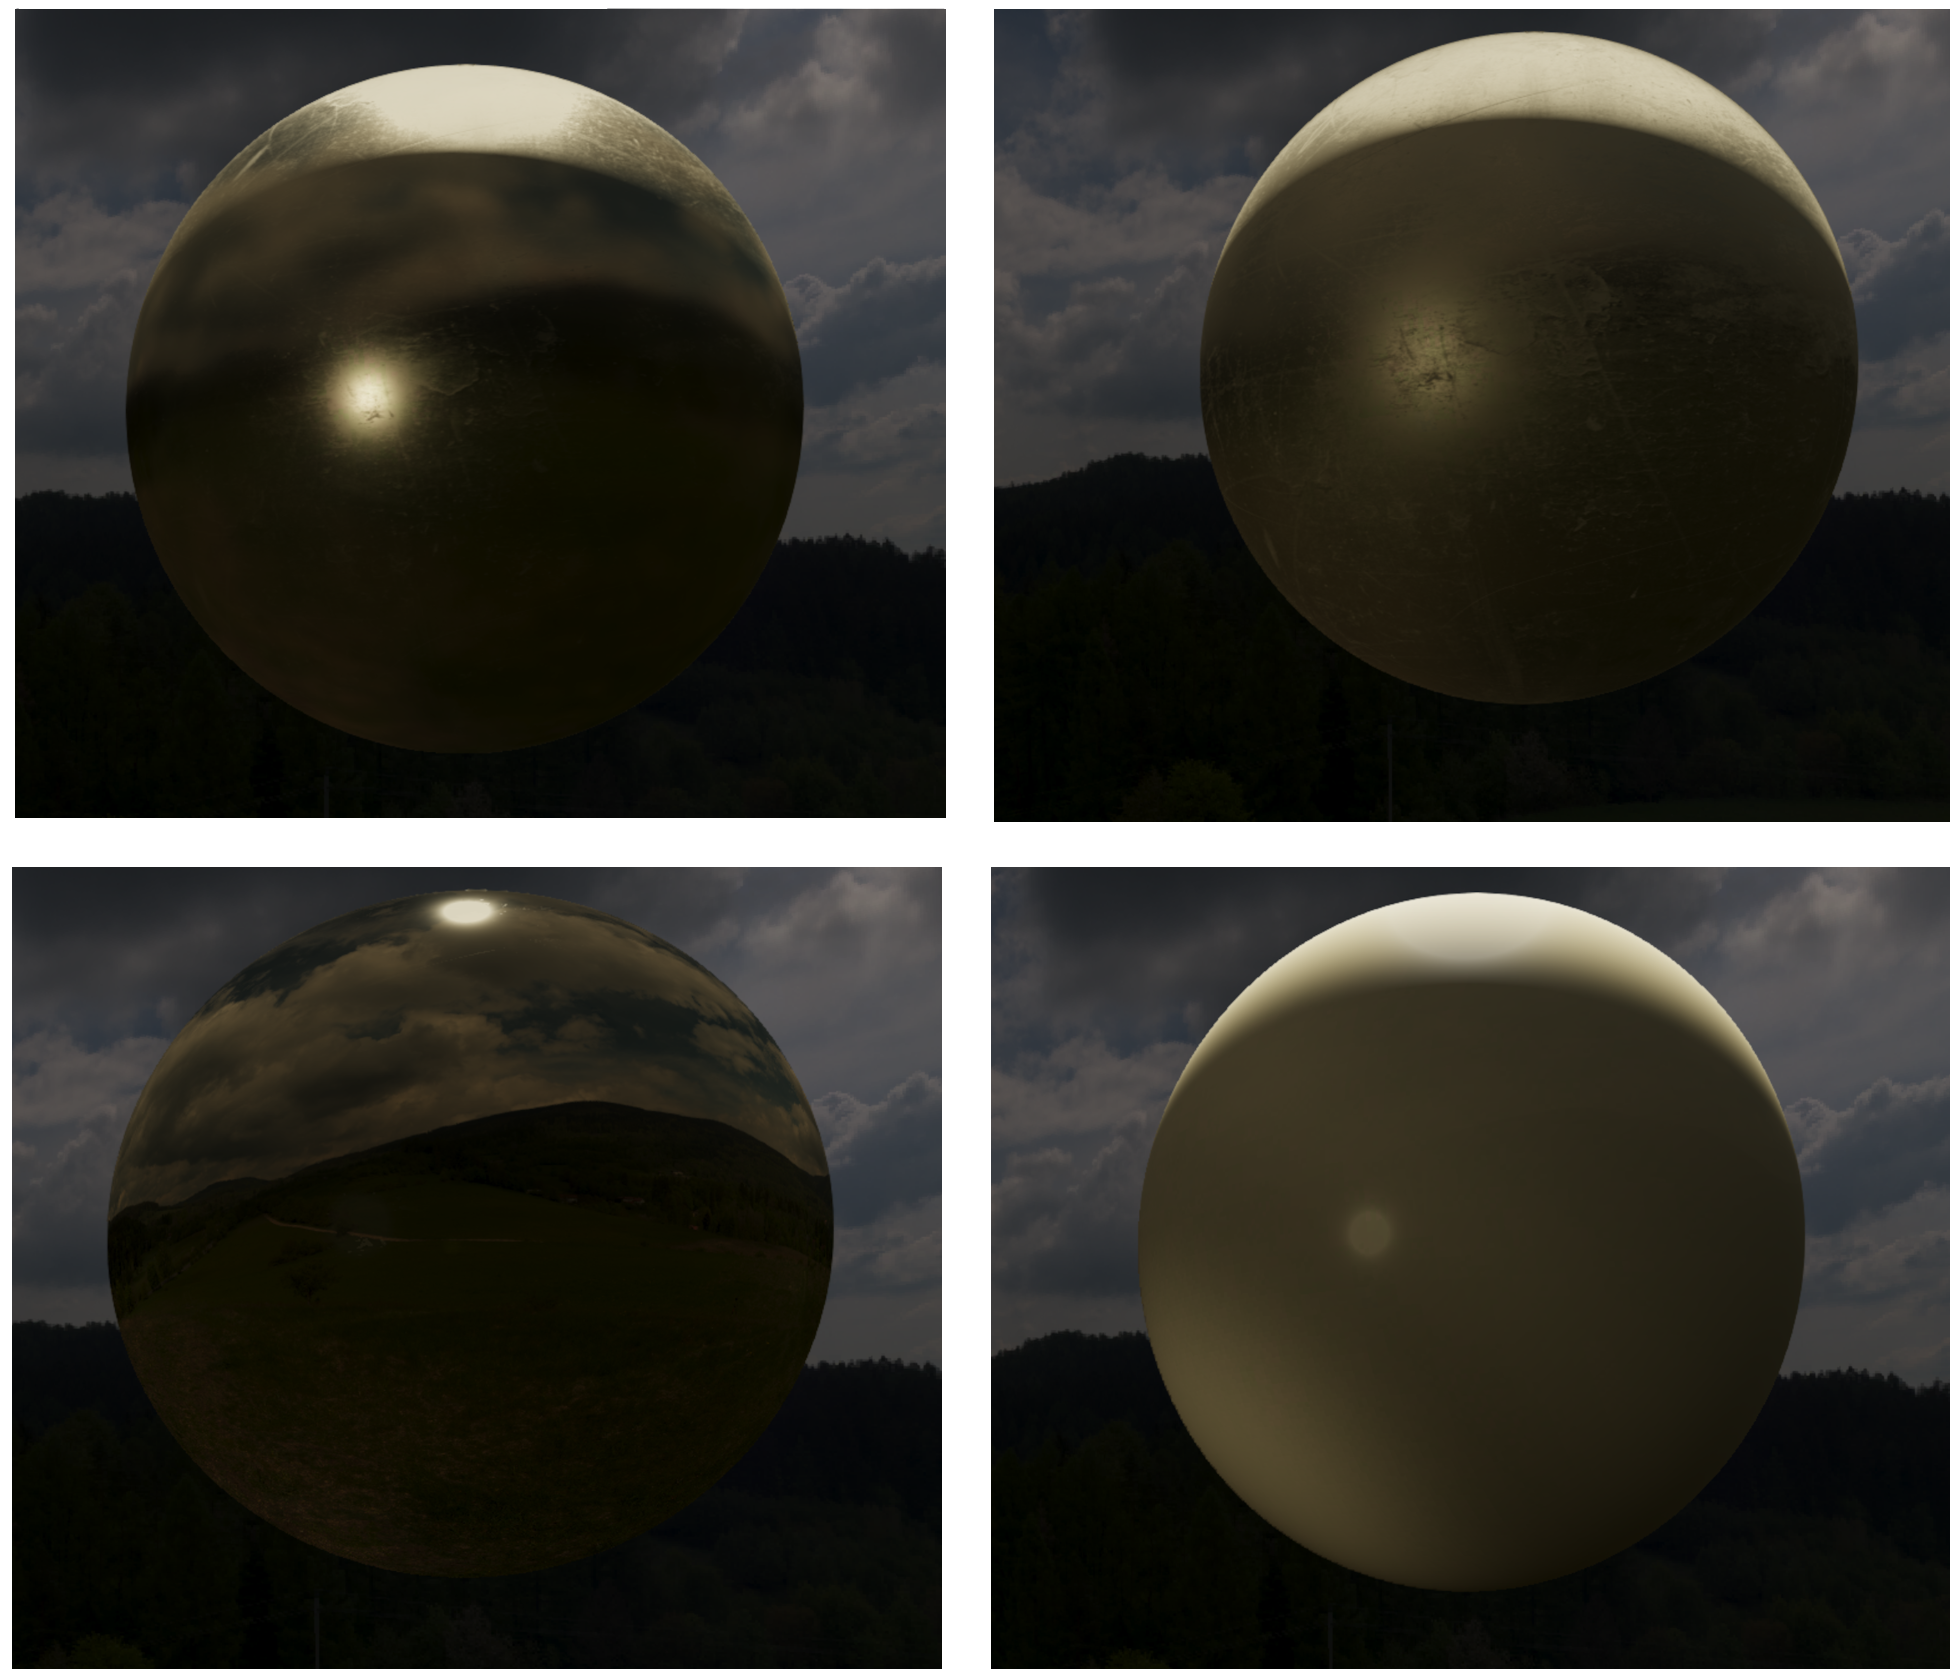
\includegraphics[width=0.8\linewidth]{Pictures/SphereComparance.png}
\caption{Порівняння вигляду сфер з різними фізичними параметрами}
\label{fig:sphere_comparison}
\end{figure}

\par Як видно з результатів, металева сфера відображає навколишнє середовище, причому ступінь розмиття відбиття прямо залежить від значення шорст\-кос\-ті: чим вище $roughness$, тим дифузнішим і менш чітким стає дзеркальне відбиття. У випадку діелектричної сфери відображення довкілля практично відсутнє; поверхня переважно демонструє дифузне розсіювання світла без характерного блиску, що відповідає фізичній поведінці неметалевих матеріалів.

\par Наступним етапом є візуалізація складнішого тривимірного об’єкта — моделі самурая (рис.~\ref{fig:samurai_full}). Зображення наведено поетапно, із поступовим відключенням окремих складових освітлення, з метою наочної демонстрації їх внеску у фінальне зображення:

\begin{enumerate}
\item Повна модель з активованими всіма компонентами освітлення (diffuse + specular).
\item Лише дифузна складова — демонструє розсіювання світла поверхнею.
\item Лише дзеркальна (specular) складова — ілюструє відбиття світла відповідно до мікрофасеткової моделі.
\end{enumerate}

\begin{figure}[h]
\centering
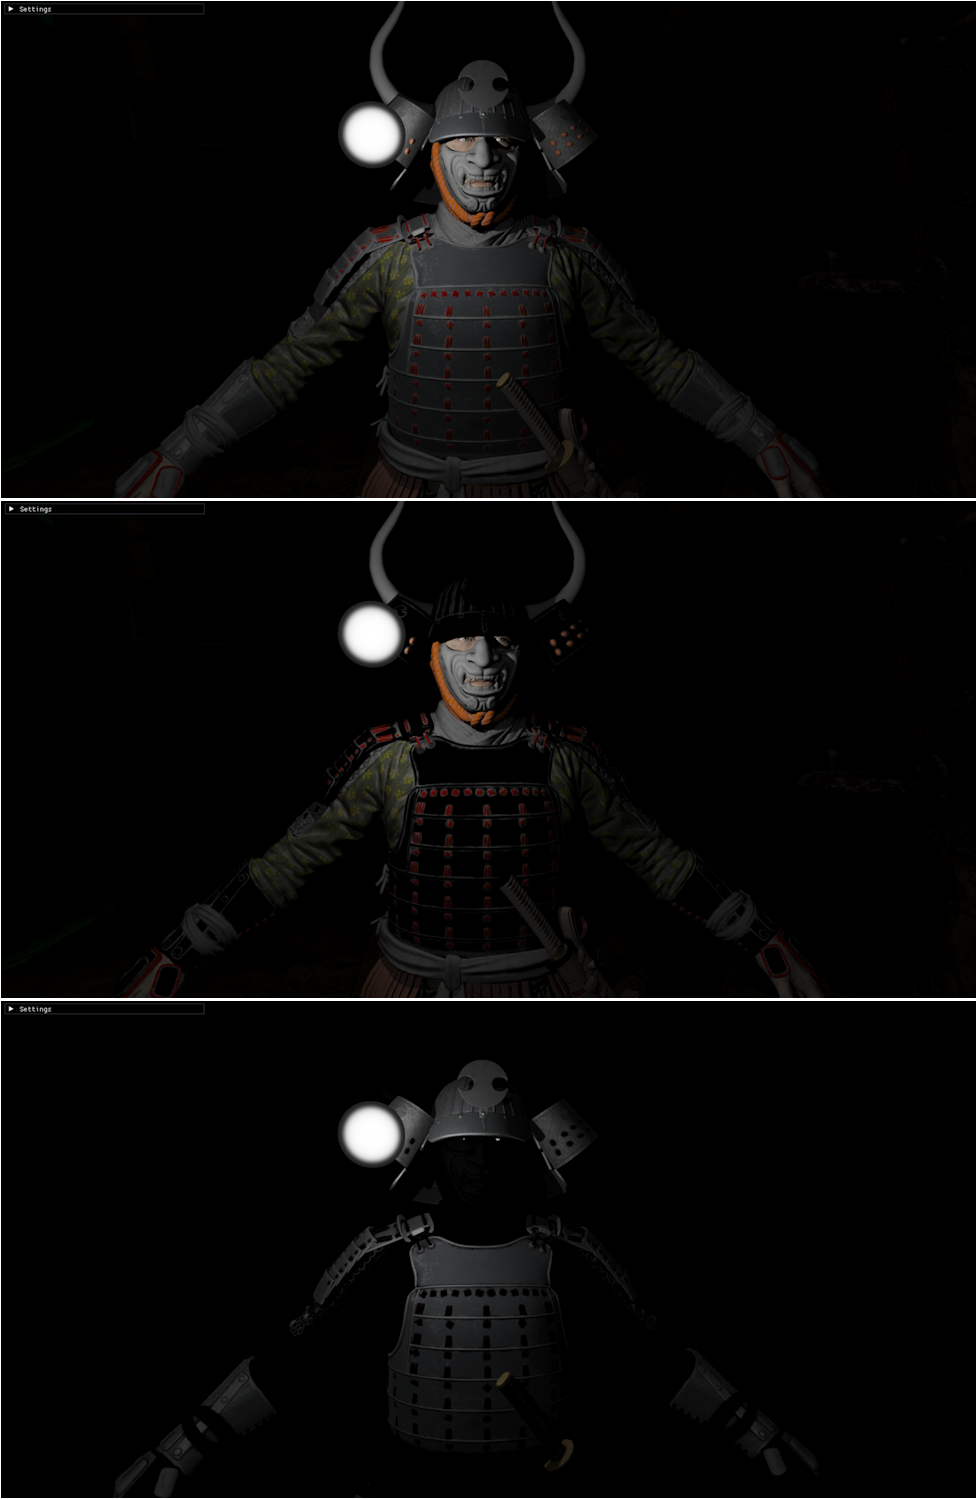
\includegraphics[scale=0.35]{Pictures/Samuraifull.png}
\caption{Порівняння вигляду моделі самурая при різних конфігураціях освіт\-лен\-ня}
\label{fig:samurai_full}
\end{figure}

\par Як видно з результатів (рис. \ref{fig:samurai_full}), при візуалізації лише дифузної складової металічні поверхні втрачають колір та виглядають тьмяно. Це пояснюється тим, що згідно з фізичними властивостями металів, дифузна складова майже повністю відсутня -- більшість світла або поглинається, або дзеркально відбивається. Навпаки, при візуалізації лише дзеркальної складової поверхні ді\-елект\-ри\-ків виглядають майже повністю темними, оскільки для них дзеркальна компонента є дуже слабкою.

\par Таким чином, проведені числові експерименти підтверджують коректність реалізованої моделі фізично обґрунтованого освітлення та її відповідність очікуваній фізичній поведінці матеріалів при різних параметрах. Отримані результати демонструють узгодженість моделі з фундаментальними законами оптики, зокрема законом збереження енергії, ефекту Френеля та властивостями мікрофасеткових відбиттів, що проявляється у правильному відтворенні таких явищ, як розмиття дзеркальних рефлексій при збільшенні шорсткості, слабке відбиття у діелектриків та кольорове віддзеркалення у металів. Це вказує на адекватність математичного апарату, використаного при дискретизації рівняння рендерингу та BRDF-моделі, а також підтверджує ефективність програмної реалізації в умовах складних сцен. Крім того, результати ілюструють високу якість візуалізації, яка досягається за рахунок правильного врахування геометричних, спектральних та освітлювальних параметрів при моделюванні.

% ***************************************************************************
 \chapter*{ВИСНОВКИ}
\par У цій кваліфікаційній роботі було здійснено комплексне дослідження тео\-ре\-тич\-них засад та практичної реалізації фізично коректного рендерингу (Phy\-si\-cal\-ly Based Rendering, PBR) у контексті тривимірної графіки та реального часу. Ос\-нов\-ною метою роботи було детальне вивчення сучасних моделей ос\-віт\-лен\-ня та матеріалів, а також побудова власного рендерера на основі графічного API DirectX~11 з підтримкою PBR-підходу.

\par Теоретична частина роботи зосереджена на фундаментальних поняттях розподілу світлових енергій у сцені, які описуються формальним рівнянням рендерингу. Було розглянуто властивості поверхонь на мікрорівні, зокрема мікрофасеткову модель відбиття світла, яка лежить в основі BRDF-функцій (Bi\-di\-rec\-tio\-nal Reflectance Distribution Function). Значну увагу приділено моделі Кука–Тор\-рен\-са, що поєднує у собі геометричну функцію видимості, розподіл нормалей поверхні (наприклад, GGX), а також ефект Френеля.

\par Крім того, розглянуто поділ матеріалів на метали та діелектрики, їхні відмінності у взаємодії з падаючим випромінюванням, а також роль таких параметрів, як металічність (metalness) та шорсткість (roughness). Описано особ\-ли\-вос\-ті дифузної  та дзеркальної  компонент відбиття, що забезпечують реаліс\-тич\-ну поведінку поверхні під різними кутами огляду та освітлення. 

\par У практичній частині реалізовано повноцінну систему PBR-рендерингу за допомогою DirectX~11. Було створено систему ресурсів для зчитування карт шорсткості, нормалей, металічності та албедо, організовано ефективну архі\-тек\-ту\-ру шейдерів, включно з модулем попередньої фільтрації environment map, а також генерації BRDF LUT для збереження продуктивності. Рендеринг виконувався за допомогою відкладеного затінювання (deferred shading), що дозволило ефективно обчислювати вплив освітлення для великої кількості пікселів одночасно.

\par У розділі чисельних експериментів було проведено серію візуальних досліджень, що демонструють поведінку матеріалів під впливом зміни параметрів PBR-моделі. Зокрема:
\begin{itemize}
    \item порівняння металічної сфери з різною шорсткістю (від ідеально гладкої до майже матової), що продемонструвало ефекти розмитого та чіт\-ко\-го дзеркального відбиття;
    \item демонстрація діелектричної сфери, де присутня лише дифузна складова без видимого дзеркального компоненту, що підтвердило правильність обчислення моделей матеріалів;
    \item пошарове відображення 3D-моделі самурая з різними компонентами освітлення (повне, лише дифузне, лише дзеркальне), що дозволило візуально оцінити внесок кожної складової BRDF-функції.
\end{itemize}

\par Усі отримані результати підтверджують правильність та ефективність реа\-лізованого підходу. Візуалізація об’єктів відповідає фізичним очікуванням й узгоджується з теоретичними моделями, що були розглянуті у попередніх розділах. Побудований рендерер продемонстрував здатність забезпечувати високу якість зображення при збереженні продуктивності в реальному часі.

\par У перспективі, розроблену систему можна розширити шляхом:
\begin{itemize}
    \item додавання глобального освітлення (Global Illumination) за допомогою технік, таких як Voxel Cone Tracing або Screen Space GI;
    \item інтеграції трасування променів у реальному часі (Ray Tracing), зокрема для обробки тіней, відбиттів та прозорості;
    \item моделювання підповерхневого розсіювання (Subsurface Scattering) для матеріалів на зразок шкіри або воску.
\end{itemize}

% ***************************************************************************
  \markright{\underline
 {\it Список використаних джерел}}
 \addcontentsline{toc}{chapter}{Список використаних джерел}

% \large
 \renewcommand{\bibname}{{Список використаних джерел}}
 \begin{thebibliography}{}
 \setcounter{theorem}{0}

 \bibitem{Ch0}
  Сеньо П. С. Теорія ймовірностей та математична статистика / П. С. Сеньо - Київ : Знання, 2007. - 556 c.

  \bibitem{Ch1}
  The Colorimetric Properties of the Spectrum. 
  Philosophical Transactions of the Royal Society of London. Series A, Containing Papers of a Mathematical or Physical Character,
  Vol. 230 (1932), pp. 149-187 (39 pages)

  \bibitem{Ch2}
    CIE 1931 color space [Електронний ресурс]. – Режим доступу: \url{https://en.wikipedia.org/wiki/CIE_1931_color_space}.

   
  \bibitem{Ch3}
  Iosifidis A. Deep Learning for Robot Perception /  A. Iosifidis, A. Tefas - U.S: Academic Press, 2022. - 634 c.
    
    \bibitem{Ch4}
    UNDERSTANDING GAMMA CORRECTION [Електронний ресурс]. – Режим доступу: \url{https://www.cambridgeincolour.com/tutorials/gamma-correction.htm}.

    \bibitem{Ch5}
    UNDERSTANDING GAMMA CORRECTION [Електронний ресурс]. – Режим доступу: \url{https://www.cambridgeincolour.com/tutorials/gamma-correction.htm}.

    \bibitem{Ch6}
    Wikipedia. Partially Observable Markov Decision Process [Електронний ресурс]. – Режим доступу: \url{https://en.wikipedia.org/wiki/Partially_observable_Markov_decision_process}.

    \bibitem{Ch7}
    Tutorialspoint. Python Deep Learning - Deep Neural Networks [Електронний ресурс]. – Режим доступу: \url{https://www.tutorialspoint.com/python_deep_learning/python_deep_learning_deep_neural_networks.htm}.

    \bibitem{Ch8}
    Deepchecks. Reinforcement Learning Applications: From Gaming to Real World [Електронний ресурс]. – Режим доступу: \url{https://deepchecks.com/reinforcement-learning-applications-from-gaming-to-real-world/}.

    \bibitem{Ch9}
    Pacific Northwest National Laboratory (PNNL). Explainer: Deep Reinforcement Learning [Електронний ресурс]. – Режим доступу: \url{https://www.pnnl.gov/explainer-articles/deep-reinforcement-learning}.

    \bibitem{Ch10}
    Pathmind. Deep Reinforcement Learning [Електронний ресурс]. – Режим доступу: \url{https://wiki.pathmind.com/deep-reinforcement-learning}.

    \bibitem{Ch11}
    Neptune AI. Markov Decision Process in Reinforcement Learning [Електронний ресурс]. – Режим доступу: \url{https://neptune.ai/blog/markov-decision-process-in-reinforcement-learning}.

    \bibitem{Ch12}
    Built In. Markov Decision Process [Електронний ресурс]. – Режим доступу: \url{https://builtin.com/machine-learning/markov-decision-process}.
    
    \bibitem{Ch13}
    Towards Data Science. Understanding Actor-Critic Methods [Електронний ресурс]. – Режим доступу: \url{https://towardsdatascience.com/understanding-actor-critic-methods-931b97b6df3f}.
    
    \bibitem{Ch14}
    Scholarpedia. Policy Gradient Methods [Електронний ресурс]. – Режим доступу: \url{http://www.scholarpedia.org/article/Policy_gradient_methods#:~:text=Policy%20gradient%20methods%20are%20a,cumulative%20reward)%20by%20gradient%20descent}.
    
    \bibitem{Ch15}
    LessWrong. Deep Q-Networks Explained [Електронний ресурс]. – Режим доступу: \url{https://www.lesswrong.com/posts/kyvCNgx9oAwJCuevo/deep-q-networks-explained}.
    
 \end {thebibliography}

% ***************************************************************************

% ***************************************************************************
\end{document}